%  LaTeX support: latex@mdpi.com 
%  For support, please attach all files needed for compiling as well as the log file, and specify your operating system, LaTeX version, and LaTeX editor.

%=================================================================
\documentclass[sensors,article,accept,pdftex,moreauthors]{Definitions/mdpi} 
% For posting an early version of this manuscript as a preprint, you may use "preprints" as the journal and change "submit" to "accept". The document class line would be, e.g., \documentclass[preprints,article,accept,moreauthors,pdftex]{mdpi}. This is especially recommended for submission to arXiv, where line numbers should be removed before posting. For preprints.org, the editorial staff will make this change immediately prior to posting.

%--------------------
% Class Options:
%--------------------
%----------
% journal
%----------
% Choose between the following MDPI journals:
% acoustics, actuators, addictions, admsci, adolescents, aerospace, agriculture, agriengineering, agronomy, ai, algorithms, allergies, alloys, analytica, animals, antibiotics, antibodies, antioxidants, applbiosci, appliedchem, appliedmath, applmech, applmicrobiol, applnano, applsci, aquacj, architecture, arts, asc, asi, astronomy, atmosphere, atoms, audiolres, automation, axioms, bacteria, batteries, bdcc, behavsci, beverages, biochem, bioengineering, biologics, biology, biomass, biomechanics, biomed, biomedicines, biomedinformatics, biomimetics, biomolecules, biophysica, biosensors, biotech, birds, bloods, blsf, brainsci, breath, buildings, businesses, cancers, carbon, cardiogenetics, catalysts, cells, ceramics, challenges, chemengineering, chemistry, chemosensors, chemproc, children, chips, cimb, civileng, cleantechnol, climate, clinpract, clockssleep, cmd, coasts, coatings, colloids, colorants, commodities, compounds, computation, computers, condensedmatter, conservation, constrmater, cosmetics, covid, crops, cryptography, crystals, csmf, ctn, curroncol, currophthalmol, cyber, dairy, data, dentistry, dermato, dermatopathology, designs, diabetology, diagnostics, dietetics, digital, disabilities, diseases, diversity, dna, drones, dynamics, earth, ebj, ecologies, econometrics, economies, education, ejihpe, electricity, electrochem, electronicmat, electronics, encyclopedia, endocrines, energies, eng, engproc, ent, entomology, entropy, environments, environsciproc, epidemiologia, epigenomes, est, fermentation, fibers, fintech, fire, fishes, fluids, foods, forecasting, forensicsci, forests, foundations, fractalfract, fuels, futureinternet, futureparasites, futurepharmacol, futurephys, futuretransp, galaxies, games, gases, gastroent, gastrointestdisord, gels, genealogy, genes, geographies, geohazards, geomatics, geosciences, geotechnics, geriatrics, hazardousmatters, healthcare, hearts, hemato, heritage, highthroughput, histories, horticulturae, humanities, humans, hydrobiology, hydrogen, hydrology, hygiene, idr, ijerph, ijfs, ijgi, ijms, ijns, ijtm, ijtpp, immuno, informatics, information, infrastructures, inorganics, insects, instruments, inventions, iot, j, jal, jcdd, jcm, jcp, jcs, jdb, jeta, jfb, jfmk, jimaging, jintelligence, jlpea, jmmp, jmp, jmse, jne, jnt, jof, joitmc, jor, journalmedia, jox, jpm, jrfm, jsan, jtaer, jzbg, kidney, kidneydial, knowledge, land, languages, laws, life, liquids, literature, livers, logics, logistics, lubricants, lymphatics, machines, macromol, magnetism, magnetochemistry, make, marinedrugs, materials, materproc, mathematics, mca, measurements, medicina, medicines, medsci, membranes, merits, metabolites, metals, meteorology, methane, metrology, micro, microarrays, microbiolres, micromachines, microorganisms, microplastics, minerals, mining, modelling, molbank, molecules, mps, msf, mti, muscles, nanoenergyadv, nanomanufacturing, nanomaterials, ncrna, network, neuroglia, neurolint, neurosci, nitrogen, notspecified, nri, nursrep, nutraceuticals, nutrients, obesities, oceans, ohbm, onco, oncopathology, optics, oral, organics, organoids, osteology, oxygen, parasites, parasitologia, particles, pathogens, pathophysiology, pediatrrep, pharmaceuticals, pharmaceutics, pharmacoepidemiology, pharmacy, philosophies, photochem, photonics, phycology, physchem, physics, physiologia, plants, plasma, pollutants, polymers, polysaccharides, poultry, powders, preprints, proceedings, processes, prosthesis, proteomes, psf, psych, psychiatryint, psychoactives, publications, quantumrep, quaternary, qubs, radiation, reactions, recycling, regeneration, religions, remotesensing, reports, reprodmed, resources, rheumato, risks, robotics, ruminants, safety, sci, scipharm, seeds, sensors, separations, sexes, signals, sinusitis, skins, smartcities, sna, societies, socsci, software, soilsystems, solar, solids, sports, standards, stats, stresses, surfaces, surgeries, suschem, sustainability, symmetry, synbio, systems, taxonomy, technologies, telecom, test, textiles, thalassrep, thermo, tomography, tourismhosp, toxics, toxins, transplantology, transportation, traumacare, traumas, tropicalmed, universe, urbansci, uro, vaccines, vehicles, venereology, vetsci, vibration, viruses, vision, waste, water, wem, wevj, wind, women, world, youth, zoonoticdis 

%---------
% article
%---------
% The default type of manuscript is "article", but can be replaced by: 
% abstract, addendum, article, book, bookreview, briefreport, casereport, comment, commentary, communication, conferenceproceedings, correction, conferencereport, entry, expressionofconcern, extendedabstract, datadescriptor, editorial, essay, erratum, hypothesis, interestingimage, obituary, opinion, projectreport, reply, retraction, review, perspective, protocol, shortnote, studyprotocol, systematicreview, supfile, technicalnote, viewpoint, guidelines, registeredreport, tutorial
% supfile = supplementary materials

%----------
% submit
%----------
% The class option "submit" will be changed to "accept" by the Editorial Office when the paper is accepted. This will only make changes to the frontpage (e.g., the logo of the journal will get visible), the headings, and the copyright information. Also, line numbering will be removed. Journal info and pagination for accepted papers will also be assigned by the Editorial Office.

%------------------
% moreauthors
%------------------
% If there is only one author the class option oneauthor should be used. Otherwise use the class option moreauthors.

%---------
% pdftex
%---------
% The option pdftex is for use with pdfLaTeX. If eps figures are used, remove the option pdftex and use LaTeX and dvi2pdf.

%=================================================================
% MDPI internal commands
\firstpage{1} 
\makeatletter 
\setcounter{page}{\@firstpage} 
\makeatother
\pubvolume{1}
\issuenum{1}
\articlenumber{0}
\pubyear{2022}
\copyrightyear{2022}
\externaleditor{Academic Editor: {Ahmed Bouridane} %MDPI: Please add academic editor if available.
}
\datereceived{30 August 2022} 
%\daterevised{} % Only for the journal Acoustics
\dateaccepted{23 September 2022} 
\datepublished{} 
%\datecorrected{} % Corrected papers include a "Corrected: XXX" date in the original paper.
%\dateretracted{} % Corrected papers include a "Retracted: XXX" date in the original paper.
\hreflink{https://doi.org/} % If needed use \linebreak
%\doinum{}
%------------------------------------------------------------------
% The following line should be uncommented if the LaTeX file is uploaded to arXiv.org
%\pdfoutput=1

%=================================================================
% Add packages and commands here. The following packages are loaded in our class file: fontenc, inputenc, calc, indentfirst, fancyhdr, graphicx, epstopdf, lastpage, ifthen, lineno, float, amsmath, setspace, enumitem, mathpazo, booktabs, titlesec, etoolbox, tabto, xcolor, soul, multirow, microtype, tikz, totcount, changepage, attrib, upgreek, cleveref, amsthm, hyphenat, natbib, hyperref, footmisc, url, geometry, newfloat, caption
\usepackage{makecell}
\usepackage{placeins}
\usepackage{amsmath}
\usepackage{comment}
\usepackage{soulutf8}
%\usepackage[adjustmargins]{LatexPackage/trackchanges}
%\addeditor{H.K.D}

%=================================================================
%% Please use the following mathematics environments: Theorem, Lemma, Corollary, Proposition, Characterization, Property, Problem, Example, ExamplesandDefinitions, Hypothesis, Remark, Definition, Notation, Assumption
%% For proofs, please use the proof environment (the amsthm package is loaded by the MDPI class).

%=================================================================
% Full title of the paper (Capitalized)
\Title{Skin Lesion Classification on Imbalanced Data Using Deep Learning with Soft Attention}

% MDPI internal command: Title for citation in the left column
\TitleCitation{Skin Lesion Classification on Imbalanced Data Using Deep Learning with Soft Attention}

% Author Orchid ID: enter ID or remove command
\newcommand{\orcidauthorA}{0000-0001-7152-0191} % Add \orcidA{} behind the author's name
\newcommand{\orcidauthorB}{0000-0001-9934-7474} % Add \orcidB{} behind the author's name
\newcommand{\orcidauthorC}{0000-0002-2566-5637} % Add \orcidC{} behind the author's name

% Authors, for the paper (add full first names)
\Author{{Viet} %MDPI: Please carefully check the accuracy of names and affiliations.
 Dung Nguyen $^{1,\dagger,}$*\orcidA{}, Ngoc Dung Bui $^{2,}${*} %MDPI: The correspondence author is different from the submitting system. Please confirm which one is correct.
\orcidB{} and Hoang Khoi Do  $^{1,\dagger}$\orcidC{}}

%\longauthorlist{yes}

% MDPI internal command: Authors, for metadata in PDF
\AuthorNames{Viet Dung Nguyen, Ngoc Dung Bui, and Hoang Khoi Do}

% MDPI internal command: Authors, for citation in the left column
\AuthorCitation{Nguyen, V.D.; Bui, N.D.; Do, H.K.}
% If this is a Chicago style journal: Lastname, Firstname, Firstname Lastname, and Firstname Lastname.

% Affiliations / Addresses (Add [1] after \address if there is only one affiliation.)

\address{$^{1}$ \quad {School} %MDPI: we combined the same affiliation 1 and 3, please confirm.
 of Electrical and Electronic Engineering, Hanoi University of Science and Technology, {Dai Co Viet, Ha Noi 100000, Vietnam;} %MDPI: Please add the city and post code.
{khoi.dh200322@sis.hust.edu.vn} %MDPI: This email address is different from the submitting system. Please confirm which one is correct. %H.K.D confirmed
\\
$^{2}$ \quad Faculty of Information Technology, University of Transport and Communications, {Ha Noi 115000, Vietnam} %MDPI: Please add the city and post code.
}

% Contact information of the corresponding author
\corres{Correspondences: dung.nguyenviet1@hust.edu.vn (V.D.N.); dnbui@utc.edu.vn (N.D.B.); \mbox{Tel.: +84-9834-443-22 (N.V.D.);} +84-9130-451-30 (N.D.B.)}

% Current address and/or shared authorship
\firstnote{Current address: 1st Dai Co Viet Street, {Ha Noi 100000, } %MDPI: 1. Please add the postal code. If the postal code is not available, please provide the P.O. Box. 2. If this address is the supplementary of address 1, then please combine them together. 
%H.K.D We have already provied the postal code
 Vietnam.} 
% The commands \thirdnote{} till \eighthnote{} are available for further notes 

%\simplesumm{} % Simple summary

%\conference{} % An extended version of a conference paper

% Abstract (Do not insert blank lines, i.e. \\) s
\abstract{Today, the rapid development of industrial zones leads to an increased incidence of skin	diseases because of polluted air. According to a report by the American Cancer Society, it is estimated that in 2022 there will be about 100,000 people suffering from skin cancer and more than 7600 of these people will not survive. In the context that doctors at provincial hospitals and health facilities are overloaded, doctors at lower levels lack experience, and having	a tool to support doctors in the process of diagnosing skin diseases quickly and accurately is essential. Along with the strong development of artificial intelligence technologies, many solutions to support the diagnosis of skin diseases have been researched and developed. In this paper, a combination of one Deep Learning model (DenseNet, InceptionNet, ResNet, etc) with Soft-Attention, which unsupervisedly extract a heat map of main skin lesions. Furthermore, personal information including age and gender are also used. It is worth noting that a new loss function that takes into account the data imbalance is also proposed. Experimental results on data set HAM10000 show that using InceptionResNetV2 with Soft-Attention and the new loss function gives 90 percent accuracy, mean of precision, F1-score, recall, and AUC of 0.81, 0.81, 0.82, and 0.99, respectively. Besides, using MobileNetV3Large combined with Soft-Attention and the new loss function, even though the number of parameters is 11~times less and the number of hidden layers is 4 times less, it achieves an accuracy of 0.86 and 30 times faster diagnosis than InceptionResNetV2.}

% Keywords
\keyword{{skin lesions;} %MDPI: We removed the uppercase of some keywords, please confirm  
classification; deep learning; soft-attention; imbalance} 
% Confirmed, we also removed the duplicated "skin lesions"

% The fields PACS, MSC, and JEL may be left empty or commented out if not applicable
%\PACS{J0101}
%\MSC{}
%\JEL{}

%%%%%%%%%%%%%%%%%%%%%%%%%%%%%%%%%%%%%%%%%%
% Only for the journal Diversity
%\LSID{\url{http://}}

%%%%%%%%%%%%%%%%%%%%%%%%%%%%%%%%%%%%%%%%%%
% Only for the journal Applied Sciences
%\featuredapplication{Authors are encouraged to provide a concise description of the specific application or a potential application of the work. This section is not mandatory.}
%%%%%%%%%%%%%%%%%%%%%%%%%%%%%%%%%%%%%%%%%%

%%%%%%%%%%%%%%%%%%%%%%%%%%%%%%%%%%%%%%%%%%
% Only for the journal Data
%\dataset{DOI number or link to the deposited data set if the data set is published separately. If the data set shall be published as a supplement to this paper, this field will be filled by the journal editors. In this case, please submit the data set as a supplement.}
%\datasetlicense{License under which the data set is made available (CC0, CC-BY, CC-BY-SA, CC-BY-NC, etc.)}

%%%%%%%%%%%%%%%%%%%%%%%%%%%%%%%%%%%%%%%%%%
% Only for the journal Toxins
%\keycontribution{The breakthroughs or highlights of the manuscript. Authors can write one or two sentences to describe the most important part of the paper.}

%%%%%%%%%%%%%%%%%%%%%%%%%%%%%%%%%%%%%%%%%%
% Only for the journal Encyclopedia
%\encyclopediadef{For entry manuscripts only: please provide a brief overview of the entry title instead of an abstract.}

%%%%%%%%%%%%%%%%%%%%%%%%%%%%%%%%%%%%%%%%%%
\begin{document}
	
	%%%%%%%%%%%%%%%%%%%%%%%%%%%%%%%%%%%%%%%%%%
	\setcounter{section}{0} %% Remove this when starting to work on the template.
	\begin{comment}
		\section{How to Use this Template}
		
		The template details the sections that can be used in a manuscript. Note that the order and names of article sections may differ from the requirements of the journal (e.g., the positioning of the Materials and Methods section). Please check the instructions on the authors' page of the journal to verify the correct order and names. For any questions, please contact the editorial office of the journal or support@mdpi.com. For LaTeX-related questions please contact latex@mdpi.com.%\endnote{This is an endnote.} % To use endnotes, please un-comment \printendnotes below (before References). Only journal Laws uses \footnote.
		
		% The order of the section titles is: Introduction, Materials and Methods, Results, Discussion, Conclusions for these journals: aerospace,algorithms,antibodies,antioxidants,atmosphere,axioms,biomedicines,carbon,crystals,designs,diagnostics,environments,fermentation,fluids,forests,fractalfract,informatics,information,inventions,jfmk,jrfm,lubricants,neonatalscreening,neuroglia,particles,pharmaceutics,polymers,processes,technologies,viruses,vision
	\end{comment}
	
	\section{Introduction} 
	\subsection{Problem Statement}
%	\change[H.K.D]{One of the most common malignancies that cause death globally is skin cancer. In the United States, more than 9500 persons receive a skin cancer diagnosis each day~\mbox{\cite{03358}}. The Skin Cancer Foundation reports that there is an ongoing rise in the incidence of skin cancer worldwide~\mbox{\cite{11872}}. In the United States, 192,310 new cases of melanoma are anticipated to be detected in 2019. On the other hand, if patients receive an early diagnosis, their chances of survival are 99 percent. Survival is, however, generally poor after the illness has spread beyond the skin~\mbox{\cite{11872}}. Additionally, there is a need for an efficient solution because of the rising prevalence of skin malignancies, low awareness among a population that is expanding, and a lack of sufficient clinical competence and services.}
	{Skin cancer is one of the most common cancers leading to worldwide death. {Every day, more than 9500~\mbox{\cite{03358}} }%MDPI: We adjust the number of cited reference, please check the cited reference again.
	people in the United States are diagnosed with skin cancer. Otherwise, 3.6~\mbox{\cite{03358}} million people are diagnosed with basal cell skin cancer each year. According to the Skin Cancer Foundation, the global incidence of skin cancer continues to increase~\mbox{\cite{11872}}. In 2019, it is estimated that 192,310 cases of melanoma will be diagnosed in the United States~\mbox{\cite{11872}}. On the other hand, if patients are early diagnosed, the survival rate is correlated with 99 percent. However, once the disease progresses beyond the skin, survival is poor~\mbox{\cite{11872}}. Moreover, with the increasing incidence of skin cancers, low awareness among a growing population, and a lack of adequate clinical expertise and services, there is a need for effective solutions.} 
	
	Recently, deep learning particularly, and machine learning in general algorithms have emerged to achieve excellent performance on various tasks, especially in skin disease diagnosis tasks. AI-enabled computer-aided diagnostics (CAD)\cite{11797} has solutions in three main categories: Diagnosis, Prognosis, and Medical Treatment. Medical imaging, including ultrasound, computed tomography, magnetic resonance imaging, and X-ray image is used extensively in clinical practice. In Diagnosis, Artificial Intelligence (AI) algorithms are applied for disease detection to save progress execution before these diagnosis results are considered by a doctor. In Prognosis, AI algorithms are used to predict the survival rate of a patient based on his/her history and medical data. In Medical Treatment, AI models are applied to build solutions to a specific disease; medicine revolution is an example. In various studies, AI algorithms have provided various end-to-end solutions to the detection of abnormalities such as breast cancer, brain tumors, lung cancer, esophageal cancer, skin lesions, and foot ulcers across multiple image modalities of medical imaging \cite{11872}.
	
	To adapt the rise in skin cancer cases, AI algorithms over the last decade has a great performance. Some typical models that can be mentioned are DenseNet \cite{06993}, EfficientNet  ~\cite{04861}, Inception  \cite{00567,07261}, MobileNets \cite{04861,04381,02244}, {Xception \mbox{\cite{02357}}}, ResNet \cite{03385,05027}, and NasNet   \cite{07012}. Some of these models which have been used as a backbone model in this paper will be discussed in the Related Work section.
	
	\subsection{Related Works}
%	\change[H.K.D]{Skin lesion classification is not a new area, since there are many great performance models constructed. One of the most cutting-edge technologies that have been used is Soft-Attention as stated in~\mbox{\cite{03358}}. Soumyyak~et~al. construct several models formed by the combination of a backbone model including DenseNet201~\mbox{\cite{06993}}, InceptionResNetV2~\mbox{\cite{00567}}, ResNet50~\mbox{\cite{03385,05027}}, VGG16~\mbox{\cite{1556}} and Soft-Attention layer. Their approach is to add the Soft-Attention layer at the end or the middle of the backbone model. For ResNet50 and VGG16, the Soft-Attention layer is added after the third residual block and CNN block, respectively. DenseNet201 and InceptionResNetV2, otherwise concatenate with the Soft-Attention before a fully-connected layer, and then the soft-max layer.
		
%		Using those above backbones has been tried by many previous papers. Rishu\linebreak Garg~et~al.~\mbox{\cite{03798}} uses transfer learning approach with CNN based model: ResNet50 and VGG16 which are pretrained with ImageNet data set. Besides, they also use data augmentation to avoid the imbalance of the data set. Histogram Equalization is also used to increase the contrast of the skin lesions before feeding into the Machine Learning algorithms including Random Forest, XGBoost, Support Vector Machine.	
		
%		Amirreaza~et~al.~\mbox{\cite{10348}} do not only use those above backbone model but also used InceptionV3~\mbox{\cite{00567}} model. In that research, the dataset HAM10000 and $PH^2$ are combined to create a 8 classes data set. Before feeding into the Deep CNN models, the image is resized to (224, 224) for DenseNet201, ResNet152, InceptionResNetV2 and (229, 229) for InceptionV3. 
		
%		Another paper that uses the backbone models is~\mbox{\cite{09418}}, Hemanth~et~al. decide to use EfficientNet~\mbox{\cite{11946}} and SeNET~\mbox{\cite{01507}} instead and CutOut~\mbox{\cite{04552v2}} method which involves creating holes of different sizes on the images i.e. technically making a random portion of image inactive during data augmentation process. 
		
%		Otherwise, Ref.~\mbox{\cite{01284}} also used Deep Convolution Neural Network, Peng Yao~et~al. used RandArgument which crops an image into several images from a fixed size, DropBlock which is used for regularization, Multi-Weighted New Loss which is used for dealing with the imbalanced data problem, end-to-end Cumulative Learning Strategy which can more effectively balance representation learning and classifier learning without additional computational cost. 
		
%		Another state of the art is GradCam and Kernel SHAP~\mbox{\cite{06612}}, Kyle Young~et~al. create model agnostic, local interpretable methods that can highlight pixels that the trained network deems relevant for the final classification. In that research they use three data sets containing HAM10000, BCN-20000 and MSK. Before feeding into the models, the images are preprocessed by binarized with a very low threshold to find the center of mass. 
		
%		On the other hand, there are also many state of the art whose great performance on skin lesion classification. The Student and Teacher Model is also a high performance model in 2021~\mbox{\cite{03225}}, which is created by Xiaohan Xing~et~al. as the combination of two model which share the memory with each other. Therefore, they can take full advantage of what others~learn. 
		
%		SkinLinkNet~\mbox{\cite{12602}} and WonderM~\mbox{\cite{03426}} are both tested the effect of segmentation on skin lesion classification problem created by Amirreza~et~al. and Yeong Chan~et~al., respectively. In WonderM, the method used is padding the image so that the image has the shape increased from (450, 600) to (600, 600). In SkinLinkNet, instead resize the image down to (448, 448). Both of SkinLinkNet and WonderM use UNet to do the segmentation task, though they use EfficientNetB0 and DenseNet to do the classification task, respectively. 
		
%		Another approach is using metadata including gender, age, and capturing position as stated in~\mbox{\cite{03910}} by Nil Gessert~et~al. The metadata is fed into fully connected neural network after being encoded into one-hot vector. All missing data point of age is set to 0. To overcome the missing data problem, the research apply one-hot encoding to the group but the initial validation is poor performance then numerical encoding is applied.
		
%		On the other hand, skin lesion classification problems are not only applied by Deep Learning but also Machine Learning. Random Forest, XGBoost, and Support Vector Machines are tested by~\mbox{\cite{03798}} of Rishu Garg~et~al. Besides, Isolation Forest is applied before the soft-max activation of the deep learning model to detect out-of-distribution skin lesion images as stated in~\mbox{\cite{10348}} by Amirreza Rezvantalab~et~al. Matrix Transformation, besides is also applied before the soft-max activation function in~\mbox{\cite{05045}} by Michele Alberti~et~al. } 
	
	{Skin lesion classification is not a new area, since there are many great performance models constructed, recent years. The skin classification approaches can be divided into two main approaches: Deep Learning and Machine Learning. Both approaches gain great performance. Data Augmentation and Feature Extractor, otherwise are two main supporters that make the model better.
		\begin{table}[H]
\caption{{Summary of related} %MDPI: we updated the format of all tables, please confirm the change. Please cite the table in the text and ensure the first citation of each table appears in numerical order. %H.K.D We also changed the table caption
works.}
\label{table:related-work-summary}

\begin{adjustwidth}{-\extralength}{0cm}
%\centering %% If there is a figure in wide page, please release command \centering
\centering
\begin{tabular}{ c  p{1.8cm}  p{1.8cm}  p{2.55cm}  p{1.5cm}  p{5cm}  p{2cm} }
	\toprule
	\textbf{Work} & \textbf{Deep Learning} & \textbf{Machine Learning} & \textbf{Data\linebreak Augmentation} & \textbf{Feature Extractor} & \textbf{Data Set} & \textbf{Result}\\
	\midrule
	\cite{03358} & Classify & & x & & HAM10000 & 0.93 (ACC)\\
	\midrule
	\cite{03798} & Classify & Classify & x & x & HAM10000 & 0.9 (ACC)\\
	\midrule
	\cite{10348} & Classify & Classify & x & & HAM10000, $PH^2$ & \\
	\midrule
	\cite{09418} & Classify & & x & & HAM10000 & 0.88 (ACC)\\
	\midrule
	\cite{01284} & Classify & & x & & HAM10000 & 0.86 (ACC)\\
	\midrule
	\cite{06612} & Classify & & x & x & HAM10000, BCN-20000, MSK & 0.85 (ACC)\\
	\midrule
	\cite{03225} & Classify & & x & & HAM10000 & 0.85 (ACC)\\
	\midrule
	\cite{12602} & Classify & & x & & HAM10000 & 0.92 (AUC)\\
	\midrule
	\cite{03426} & Classify & & x & & HAM10000 & 0.92 (AUC)\\
	\midrule
	\cite{03910} & Classify & & x & & HAM10000 & 0.74 (recall)\\
	\midrule
	\cite{05045} & & Classify & x & x & HAM10000 & \\
	\midrule
	\cite{2101.133} & Classify&  & x &  & HAM10000 & 0.92 (ACC)\\
	\midrule
	\cite{22750} & Seg&  &  &  & HAM10000 & 0.99 (ACC)\\
	\midrule
	\cite{9445180} & Seg &  &  &  & HAM10000 & 0.97 (ACC)\\
	\bottomrule
\end{tabular}
\end{adjustwidth}
		\end{table}
		\subsubsection{Deep Learning Approach}
		In Deep Learning, one of the most cutting-edge technologies  used is Soft-Attention, as stated in~\mbox{\cite{03358}}. Soumyyak~et~al. constructed several models formed by a combination of a backbone model including DenseNet201~\mbox{\cite{06993}}, InceptionResNetV2~\mbox{\cite{00567}}, ResNet50~\mbox{\cite{03385,05027}}, VGG16~\mbox{\cite{1556}} and Soft-Attention layer. Their approach adds the Soft-Attention layer at the end or the middle of the backbone model. For ResNet50 and VGG16, the Soft-Attention layer is added after the third residual block and CNN block, respectively. DenseNet201 and InceptionResNetV2 then concatenate with  Soft-Attention before a fully-connected layer and then soft-max layer. Soumyyak~et~al.'s proposed method gained great performances and also outperformed many other studies with an accuracy of 0.93 and a precision of 0.92. However, using  data augmentation on an imbalanced dataset resulted in subpar classification  classify with respect to the  classes; therefore, their model obtained a  recall and F1-score of 0.71 and 0.75, respectively. In this research, our proposed method also considers this problem and solves it.
		
		Using the above-mentioned backbones has been attempted previously. Rishu Garg~et~al. \mbox{\cite{03798}} used a transfer learning approach with a CNN-based model: ResNet50 and VGG16 which are pretrained with an ImageNet data set. In addition, they also use data augmentation to avoid an imbalance occurring in  the data set. Histogram equalization is also used to increase the contrast of  skin lesions before being fed into machine learning algorithms including Random Forest, XGBoost, and Support Vector Machine. Histogram equalization can be considered as a heat map that takes the main feature as the number of occurrences of the same value pixel. This approach also gain great performances with an accuracy of 0.90 and  precision of 0.88. However, this approach can be biased since only one skin image of the dataset contains the skin lesion at the center and the background skin, and the histogram may treat the background with increased numbers of occurrence with respect to the same pixel value. In this research study, our proposed method used  Soft-Attention, which can create a heat map feature of the lesion. Otherwise, Rishu Garg~et~al.'s proposed method also faced the problem of imbalanced classification due to an imbalanced dataset with the F1-score and recall at 0.77 and 0.74, respectively.
		
		Instead of using the entire imbalanced data set, Abayomi-alli~et~al. decided to separate the dataset into two subsets: one contains only melanoma and the other one contains the rest~\mbox{\cite{2101.133}}. Before feeding the data to classify  melanoma, training data are then augmented by the SMOTE method. SMOTE creates artificial instances by oversampling the minority class. SMOTE recognizes k-minority class neighbors that are near  each minority class sample by using the covariance matrix. This approach obtained an accuracy, recall, and F1-score of 0.92, 0.87, and 0.82, respectively.
		
		Amirreaza~et~al.~\mbox{\cite{10348}} did not only use the backbone model mentioned above but also used the InceptionV3~\mbox{\cite{00567}} model. In this research study,  datasets HAM10000 and $PH^2$ are combined to create an eight-class dataset. Before being fed into  Deep CNN models, the image was resized to (224, 224) for DenseNet201, ResNet152, InceptionResNetV2, and (229, 229) for InceptionV3. The best AUC values for melanoma and basal cell carcinoma are 0.94 (ResNet152) and 0.93 (DenseNet201).
		
		Another paper that uses  backbone models is~\mbox{\cite{09418}},  in which Hemanth~et~al. decided to use EfficientNet~\mbox{\cite{11946}} and SeNET~\mbox{\cite{01507}} instead and the CutOut~\mbox{\cite{04552v2}} method, which involves creating holes of different sizes on  images, i.e., technically making a random portion of image inactive during the data augmentation process. Although this approach obtained an accuracy of 0.88, it may be biased due to the CutOut method since this method can create a hole overlap in the skin lesion field. The method's accuracy is also low due to the data-augmentation process. 
		
		Otherwise, Ref.~\mbox{\cite{01284}} also used a Deep Convolution Neural Network, and Peng Yao~et~al. used RandArgument, which crops an image into several images from a fixed size; DropBlock, which is used for regularization, Multi-Weighted New Loss, which is used for dealing with the imbalanced data problem; end-to-end Cumulative Learning Strategy, which can more effectively balance representation learning; and classifier learning, without additional computational costs. This approach obtained an accuracy of 0.86. Although this approach figureed out the data imbalance problem, the result of obtaining a low accuracy may due to  RandArgument. If the skin lesion part of the image is quite big or  small, the cropped image may only contain  skin or the lesion is spread out in the entire image.
		
		{Another state-of-the-art method is GradCam and Kernel SHAP~\mbox{\cite{06612}}. Kyle Young~et~al. created an agnostic model, which includes local interpretable methods that can highlight pixels that the trained network deems relevant for the final classification. In that research study, they used three datasets containing HAM10000, BCN-20000, and MSK. Before feeding into the models,  images are preprocessed by binarization with a very low threshold to find the center of mass. This approach obtained an  AUC of 0.85.} %Please check if meaning is retained. %V.D.N confirmed
		
		On the other hand, there are also many state-of-the-art methods with great performance on skin lesion classification. The Student-and-Teacher Model is also a high-performance model introduced in 2021~\mbox{\cite{03225}}, and it is created by Xiaohan Xing~et~al. as a combination of two models that share  memories with the other model. Therefore, the models can take full advantage of what others learn. The Student-and-Teacher model obtained an accuracy of 0.85; however, the precision and F1-score are quite low, resulting in a value of 0.76.
		
		SkinLinkNet~\mbox{\cite{12602}} and WonderM~\mbox{\cite{03426}} are both tested the effect of segmentation on skin lesion classification problems created by Amirreza~et~al. and Yeong Chan~et~al., respectively. In WonderM, the method used is to pad the image so that the image has an increase in shape  from (450, 600) to (600, 600). In SkinLinkNet,  the image is instead resized down to (448, 448). Both  SkinLinkNet and WonderM used UNet to perform the segmentation task, although they used EfficientNetB0 and DenseNet to perform the classification task. This approach obtained an AUC of 0.92.
		
		Another approach is to use metadata, including gender, age, and capturing positions, as stated in~\mbox{\cite{03910}} by Nil Gessert~et~al.  Metadata are fed into a fully connected neural network after  encoded into a one-hot vector. All missing data points with respect to age are set to 0. To overcome the missing data problem, the research study applied one-hot encoding to the group, but the initial validation resulted in poor performance then when numerical encoding was applied. The metadata are then fed into two block networks, each one containing a Dense Layer, Batch Normalization, am ReLU activation function, and a Dropout. After all the feature vectors were extracted, the image was then concatenated with the feature vector extracted from metadata. Otherwise,  data augmentation was also applied. This approach obtained a  recall of 0.74. The low recall may be due to the imbalanced data set.
		
		Abnormal, skin lesion segmentation, on the other hand, also plays an important role in skin lesion classification. Nawaz~et~al. created a framework for Melanoma segmentation~\mbox{\cite{22750}}. Their proposed method is a Unet model but used  DenseNet77 as the  backbone, and all residual blocks were changed into dense block, which contains a sequence of Convolution and  Average Pooling. This melanoma segmentation approach obtain an accuracy of 0.99. Kadry~et~al. used a Unet model with a VGG deep convolution layer by pooling on the skip connection. This approach can completely extract the entire lesion, although there was an overlap observed with hair. This approach obtained an  accuracy of 0.97.
		
		\subsubsection{Machine Learning Approach}
		In Machine Learning, there are also many approaches. Since the image's data are quite complex for machine learning algorithms,  using feature extractors or feature preprocessing for transformation to another form of data is recommended.
		
		Random Forest, XGBoost, and Support Vector Machines are tested by~\mbox{\cite{03798}} of Rishu Garg~et~al. In this approach, the data are fed directly into the Machine Learning algorithm and shows no promising results; therefore, Rishu Garg~et~al. did not show the results of the used machine learning algorithm.
		
		In addition, Deep Isolation Forest is applied before the soft-max activation of the deep learning model to detect the  distribution of skin lesion images, as stated in~\mbox{\cite{09365}} by Amirreza Rezvantalab~et~al. In the Deep Isolation Forest, an feature extractor is applied by using CNN to learn the main pattern of the image. After that, the feature map is then fed into K isolation forest estimators by using bagging algorithms. The Deep Isolation Forest obtained  an accuracy of 0.9 and a confidence of 0.86. However, the AUC is only 0.74, and this may due to the limitation of the machine learning algorithm. 
		
		Matrix transformation is also applied before the soft-max activation function in~\mbox{\cite{05045}} by Michele Alberti~et~al. In this approach, the image is fed into a general model by using a sequence of residual block. The feature maps created from those above the residual block is then fed into  Global Average Pooling to create a feature vector. This feature vector is then extracted by CNN-1D and transformed by Discrete Fourier Transformation (DFT) as a filter before proceeding to the soft-max layer. 
	}
	
	\subsection{Proposed Method}
	In this research, a new model is constructed from the combination of:
	
	\begin{itemize}
	\item[-] Backbone model including DenseNet201, InceptionResNetV2, ResNet50/152, NasNetLarge, NasNetMobile, and MobileNetV2/V3;
	\item[-] Using metadata including age, gender, localization as another input of the model;
	\item[-] Using Soft-Attention as a feature extractor of the model;
	\item[-] A new weight loss function.
	\end{itemize}
	%%%%%%%%%%%%%%%%%%%%%%%%%%%%%%%%%%%%%%%%%%
	\section{Materials and Methods}
	\subsection{Materials}
	\subsubsection{Image Data}
	The data set used in this paper is the HAM10000 data set published by the Havard University Dataverse \cite{10417}. There are a total of 7 classes in this data set containing Actinic keratoses and intraepithelial carcinoma or Bowen's disease (AKIEC), basal cell carcinoma (BCC),  benign keratosis-like lesions (solar lentigines / seborrheic keratoses andchen-planus like keratoses, BKL), dermatofibroma (DF), melanoma (MEL), melanocytic nevi (NV), and vascular lesions (angiomas, angiokeratomas, pyogenic granulomas and hemorrhage, VASC). The distribution of the data set is shown in the Table \ref{table:data-distribution} below:
	
	\begin{table}[H]
		\caption{Data distribution in HAM10000.}
		\label{table:data-distribution}
		\setlength{\tabcolsep}{3.05mm}\begin{tabular}{c c c c c c c c c} 
\toprule
\textbf{Class} & \textbf{AKIEC} & \textbf{BCC} & \textbf{BKL} & \textbf{DF} & \textbf{MEL} & \textbf{NV} & \textbf{VASC} & \textbf{Total} \\ 
\midrule
No. Sample & 327 & 514 & 1099 & 115 & 1113 & 6705 & 142 & 10,015 \\
\bottomrule
		\end{tabular}
	\end{table}
	

	
	More than 50\% of lesions are confirmed through histopathology (HISTO); the ground truth for the rest of the cases is either follow-up examination (FOLLOWUP), expert consensus (CONSENSUS), or confirmation by in vivo confocal microscopy (CONFOCAL). On the other hand, before being used for training, the whole data are shuffled and then split into two parts. Here, $90$\% and $10$\% of the data is used for training and validating respectively. Images in this data set have the type of $RGB$ and shape of (450, 600). However, each backbone needs the different input sizes of images as well as the range of pixel value {(as shown in Figure \mbox{\ref{fig:data-sample}})}.
	\begin{figure}[H]
		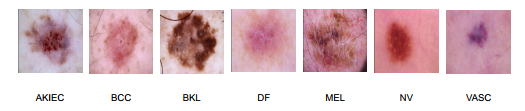
\includegraphics[width=0.8\linewidth]{Definitions/DataDistribution}
		\caption{{Example} %MDPI: 1. Please cite the figure in the text and ensure the first citation of each figure appears in numerical order. 2. Please confirm if the vertical line is necessary, if not, please remove it.
		% H.K.D We have provied the citation to the Figure 1 and feel the current version of vertical line quite great
 image of each class.}
		\label{fig:data-sample}
	\end{figure}	
	
	\subsubsection{Metadata}
	The HAM10000 data set \cite{10417} also contains the metadata of each patient including gender, age, and the capturing position, as illustrated in Table \ref{table:metadata sample}.
	\begin{table}[H]
		\caption{{Metadata}  example in the data set.}%MDPI: We remove the vertical line, please confirm. % H.K.D Confirm
		\label{table:metadata sample}
		\setlength{\tabcolsep}{11.8mm}\begin{tabular}{c c c c } 
\toprule
\textbf{ID} & \textbf{Age} & \textbf{Gender} & \textbf{Local}\\ 
\midrule
ISIC-00001 & 15 & Male & back\\
\midrule
ISIC-00002 & 85 & Female & elbow\\
\bottomrule
		\end{tabular}
	\end{table}
	\subsection{Methodology}
	\subsubsection{Overall Architecture}
	The whole architecture of the model is represented in the Figure \ref{fig:main-model}. The model takes two inputs including Image data and Metadata. The metadata branch otherwise is preprocessed before feeding into a dense layer; then, it concatenates with the output of the Soft-Attention~layer. 
	
	\begin{figure}[H]
		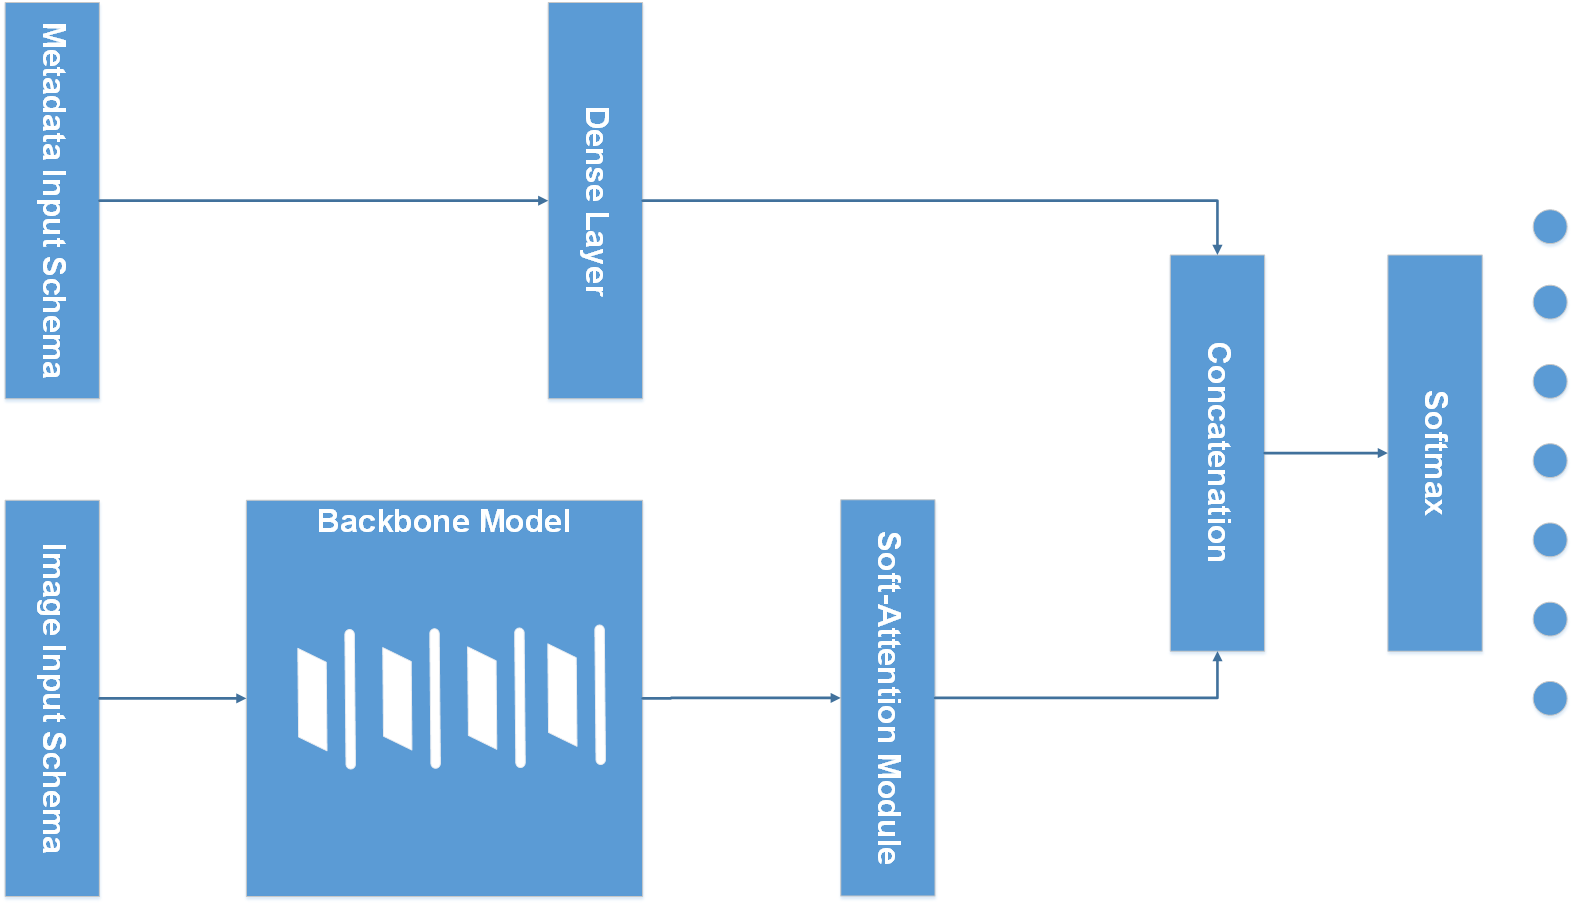
\includegraphics[width=0.9\linewidth]{Definitions/MainModel - Model Form.PNG}
		\caption{Overall model architecture.}
		\label{fig:main-model}
	\end{figure}
	
	Figure \ref{fig:model-structure} illustrates the overall structures of the combination of backbone models and Soft-Attention, which is used in this research. In detail, the combination of DenseNet201 and Soft-Attention is formed by replacing the three last (DenseBlock, Global Average Pooling, and the fully connected layer) with the Soft-Attention Module. Similarly, ResNet50 and ResNet152 also replaced the last three (Residual Block, Global Average Pooling, and the fully connected layer) with the Soft-Attention module. InceptionResNetV2, on the other hand, replaces the average pool and the last dropout with the Soft-Attention Module. The last two, Normal Cell in NasNetLarge is replaced with the Soft-Attention module. 
	
	\begin{figure}[H]
		\includegraphics[width=0.9\linewidth]{Definitions/Model  Structure.PNG}
		\caption{{Proposed} %MDPI: Please revise the "x" into a multiplication sign ("\times" U+00D7) % H.K.D confirm. %H.K.D confirmed  
 backbone model architecture. This figure show the overall structure of the backbone model (non mobile-based model) including DenseNet201, InceptionResNetV2, ResNet50, ResNet152, and NasNetLarge {with Soft-Attention}. The detailed structure and information can be found in the Appendix \ref{appendix-table:detailed structure model}.}
		\label{fig:model-structure}
	\end{figure}
	
	Figure \ref{fig:mobile-model-structure}, on the other hand, shows the detailed structure of the mobile-based mobile and its combination with Soft-Attention. All of the MobileNet versions combine with the Soft-Attention module by replacing the two last convolution layers 1 \hl{$\times$} %MDPI: We revised the "x" into a multiplication sign ("\times" U+00D7). Please confirm.
 1 with the Soft-Attention module. The NasNetMobile, otherwise, combines with the Soft-Attention module by replacing the last normal cell. 
	\begin{figure}[H]
		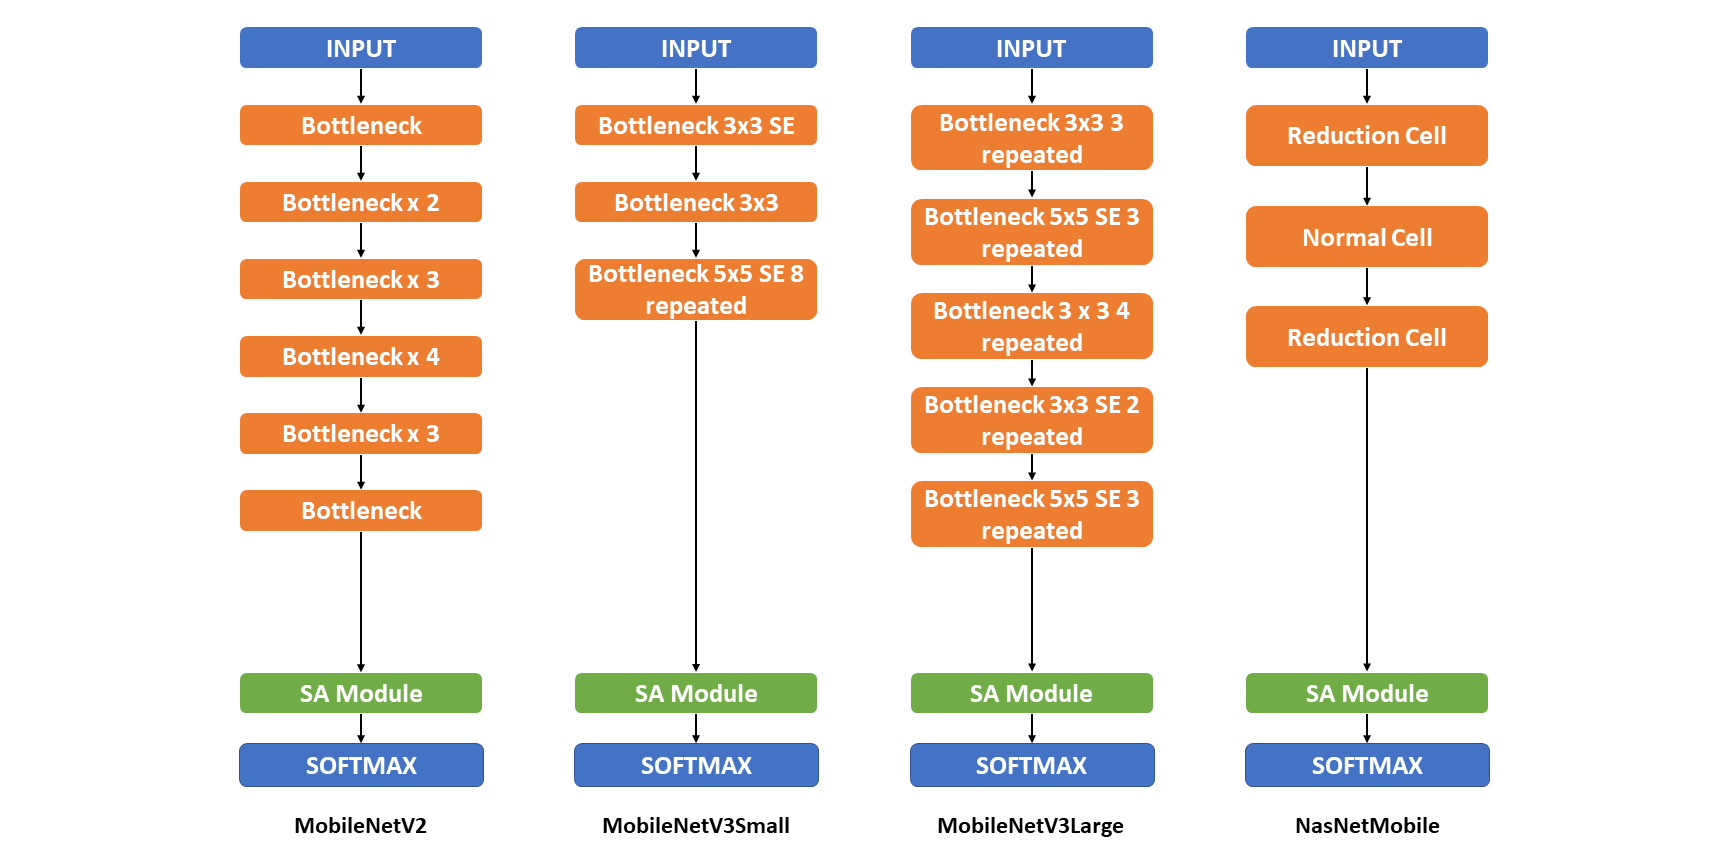
\includegraphics[width=0.9\linewidth]{Definitions/Mobile Model Structure.PNG}
		\caption{{Mobile-based} %MDPI: Please revise the "x" into a multiplication sign ("\times" U+00D7) H.K.D confirm
 backbone model architecture. This figure shows the overall structure of the mobile-based backbone model including MobileNetV2, MobileNetV3Small, MobileNetV3Large, and NasNetMobile. The detailed structure and information can be found in the Appendix \ref{appendix-table:detailed mobile model structure}.}
		\label{fig:mobile-model-structure}
	\end{figure}
	
	\subsubsection{Input Schema}
	{Image preprocessing is an essential part of the training process because of its ability to extract the main pattern of an image. In this stage, the image can be changed to the other color channel so that the main feature is separated from the useless part. Image Retrieval  has significantly created a vector that represents the main feature of an image. These image retrieval techniques can include energy compaction, primitive pattern units, etc. Shervan Fekri-Ershad~et~al. created a feature vector by calculating the element-wise product of the histogram vector in each channel of an image~\mbox{\cite{2012.4305}}}. Then, by comparing the Euclidean distance between this feature vector and the average feature vector of the entire dataset with a thresh hold, they can extract the skin portion of the image.
	
	In this research, the image data are both augmented for all classes, the number of images increases to 18,015 images , and it keeps the original form. Before feeding into the backbone model, the images are pre-processed by the input requirement of each model. DenseNet201 \cite{06993} requires the input pixels values to be scaled between $0$ and $1$ and each channel is normalized with respect to the ImageNet data set. In Resnet50 and Resnet152 \cite{03385,05027}, the images are converted from $RGB$ to $BGR$; then, each color channel is zero-centered with respect to the ImageNet data set, without scaling. InceptionResNetV2~\cite{11946}, on the other hand, will scale input pixels between $-1$ and $1$. Similarly, three versions of MobileNet \cite{04861,04381,02244}, NasNetMobile and NasNetLarge \cite{07012} require the input pixel is in range of $-1$ and $1$. 
	
	On the other hand, the metadata are also used as another input. In the research \cite{03910}, they decide to keep the missing value and set its value to $0$. The sex and anatomical site are categorically encoded. The age, on the other hand, is numerically normalized. After processing, the metadata are fed into a two-layer neural network with 256 neurons each. Each layer contains batch normalization, a ReLU \cite{08375} activation, and dropout with $p = 0.4$. The network’s output is concatenated with the CNN’s feature vector after global average pooling. Especially, they use a simple data augmentation strategy to address the problem of missing values in metadata. During training, they randomly encode each property as missing with a probability of $p = 0.1$. 
	
	In this research, the unknowns are kept as a type as discussed in the Metadata section. Sex, anatomical site, and age are also category encoded and numerically normalized, respectively. After processing, the metadata are then concatenated and fed into a dense layer of 4096 neurons. Finally, this dense layer is then concatenated with the output of Soft-Attention which is then discussed in the Soft-Attention section. The Input schema is described in {Figure} %MDPI: We changed Table to Figure. Please confirm this revision. 
	%H.K.D Great
 \ref{fig:input-schema}.
	
	\begin{figure}[H]
		\includegraphics[width=1\linewidth]{"Definitions/Input Schema"}
		\caption{Input schema.}
		\label{fig:input-schema}
	\end{figure}
	
	\subsubsection{Backbone Model}
	In this paper, the backbone models used in this paper are DenseNet201 \cite{06993}, Inception~\cite{00567}, MobileNets \cite{04861,04381,02244}, ResNet \cite{03385,05027}, and NasNet \cite{07012}. The combination of DenseNet201, InceptionResNetV2, and the Soft-Attention layer are both tested by the previous paper \cite{03358} with a great performance. Otherwise, Resnet50 also well classifies but with much fewer number of parameters and less depth than based on its F1-score and precision stated. Therefore, in this paper, the performance of the model Resnet152 and NasnetLarge models, which have more parameters and depth, is analyzed. On the other hand, three versions of MobileNet and the NasnetMobile will also be analyzed, which has fewer parameters {(as shown in Table \mbox{\ref{table:model-summary}})} and depth. 
	
	\begin{table}[H]
		\caption{{Size}, parameters, and depth of the backbone model used in this paper.}%MDPI: 1. Please cite the table in the text and ensure the first citation of each table appears in numerical order. 2. We remove the vertical line, please confirm.
		%V.D.N confirmed
		\label{table:model-summary}
		\setlength{\tabcolsep}{5.2mm}\begin{tabular}{l  c c c} 
\toprule
\textbf{Model} & \textbf{Size (MB)} & \textbf{No. Trainable Parameters} & \textbf{Depth} \\ 
\midrule
Resnet50 & 98 & 25,583,592 & 107 \\ 
\midrule
Resnet152 & 232 & 60,268,520 & 311 \\ 
\midrule
DenseNet201 & 80 & 20,013,928 & 402 \\
\midrule
InceptionResNetV2 & 215 & 55,813,192 & 449 \\
\midrule
MobileNetV2 & 14 & 3,504,872 & 105 \\ 
\midrule
MobileNetV3Small & Unknown & 2,542,856 & 88 \\ 
\midrule
MobileNetV3Large & Unknown & 5,483,032 & 118 \\
\midrule
NasnetMobile & 23 & 5,289,978 & 308 \\
\midrule
NasnetLarge & 343 & 88,753,150 & 533 \\ 
\bottomrule
		\end{tabular}
	\end{table}
	
	\subsubsection{Soft-Attention Module}
	Soft-Attention has been used in various applications: image caption generation such as \cite{03044} or handwriting verification \cite{202017}. Soft-Attention can ignore irrelevant areas of the image by multiplying the corresponding feature maps with low weights. Soft-Attention is described in {Equation}
	\eqref{eqn:softatt}. % V.D.N We update the uppercase of "Equation"
	
	\begin{equation}
		\label{eqn:softatt}
		f_{sa} = \gamma t\sum_{k=1}^{K}softmax(W_k * t)
	\end{equation}
	
	Figure \ref{fig:soft-attention} shows the two main steps of applying Soft-Attention. Firstly, the input tensor is put in grid-based feature extraction from the high-resolution image, where each grid cell is analyzed in the whole slide to generate a feature map \cite{08513}. This feature map called $t \in R^{h \times w \times d}$ where $h, w, \text{and } d$ is the shape of tensor generated by a Convolution Neural Network (CNN), is then input to a 3D convolution layer whose weights are $W_k \in R^{h \times w \times d \times K}$. The output of this convolution is normalized using the soft-max function to generate {\textit{K}} %MDPI: Please change the forward italics of the variables in the text and formulas to be consistent
	% H.K.D We have the changed the "K" into italics form
 (a constant value) attention maps. These $\textit{K}$ attention maps are aggregated to produce a weight function called $\alpha$. This $\alpha$ function is then multiplied with feature tensor $t$ and scaled by $\gamma$, which is a learnable scalar. Finally, the output of the Soft-Attention function $f_{sa}$ is the concatenation of the beginning feature tensor $t$ and the scaled attention maps. 
	
	\begin{figure}[H]
		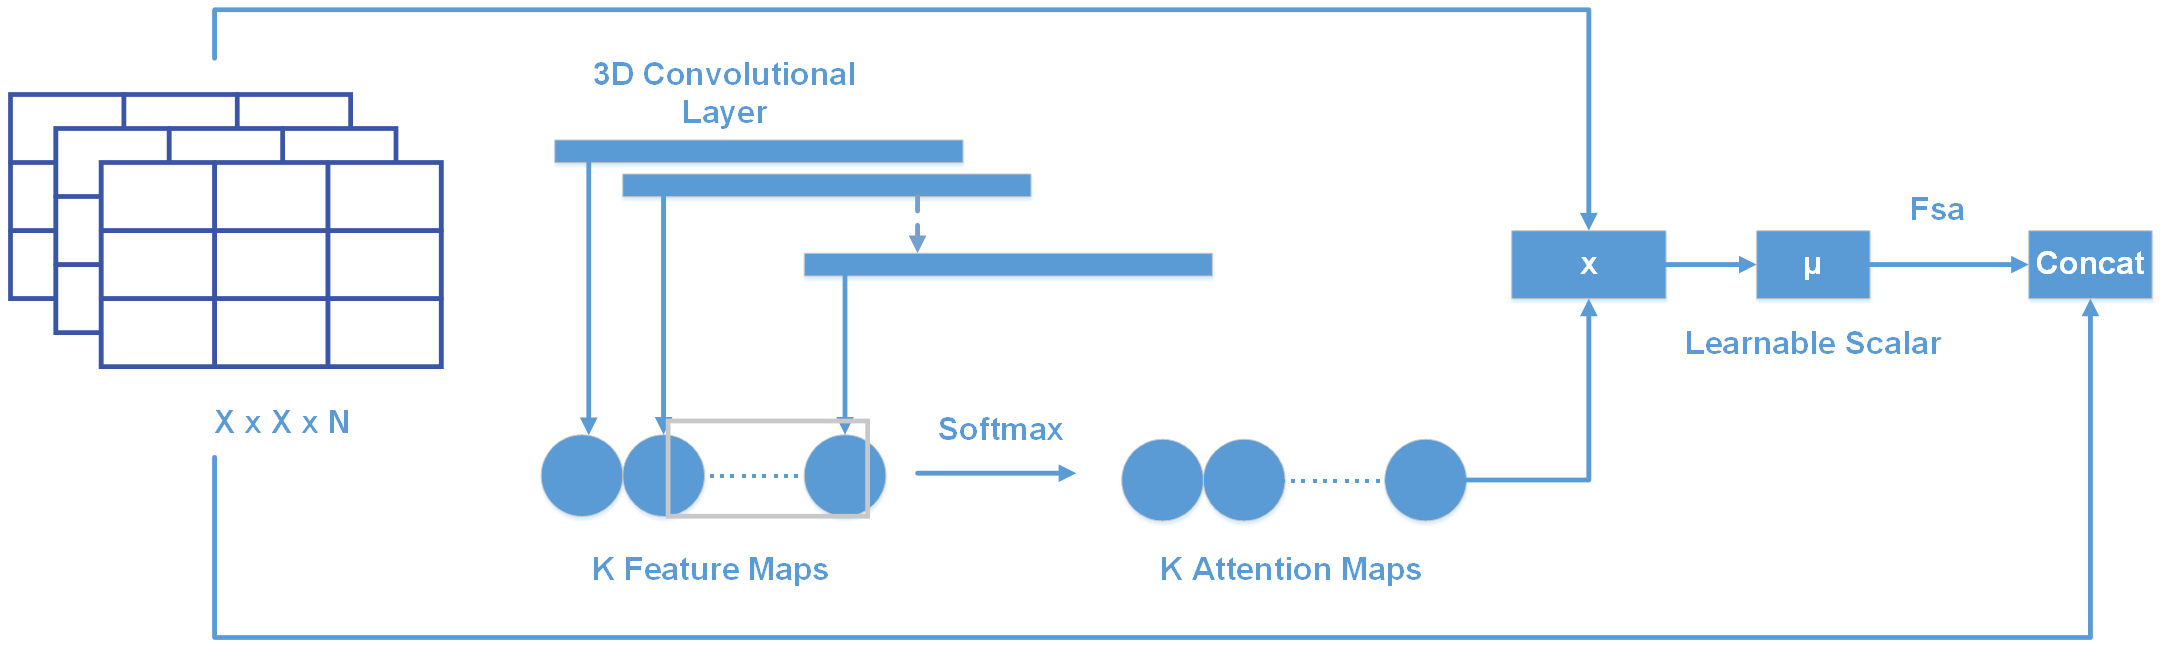
\includegraphics[width=1\linewidth]{Definitions/SoftAttention}
		\caption{{Soft-Attention layer.} %MDPI: Please revise the "*" into a multiplication sign ("\times" U+00D7) 
}
		\label{fig:soft-attention}
	\end{figure}
	
	In this research, the Soft-Attention layer is applied in the same way in \cite{03358}. The Soft-Attention module is described in Figure \ref{fig:soft-attention-block}. 
	
	\begin{figure}[H]
		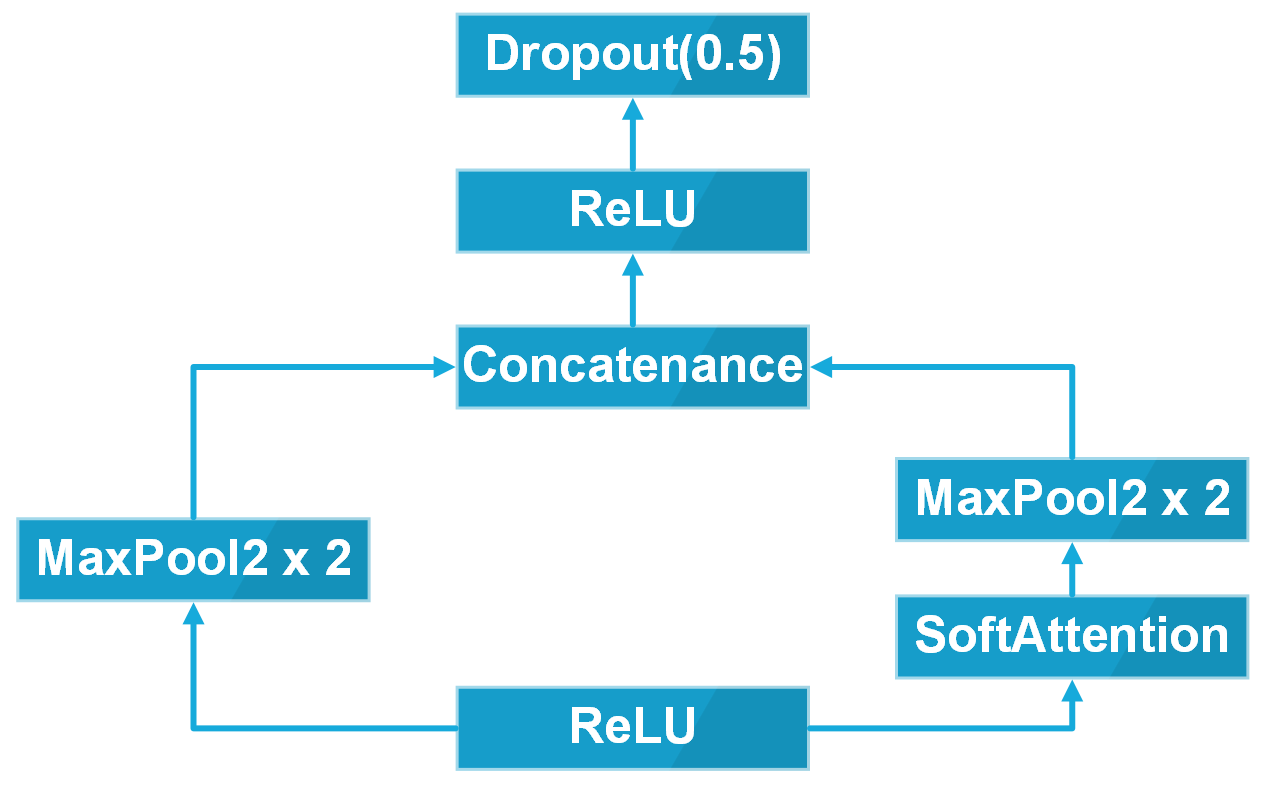
\includegraphics[width=0.5\linewidth]{Definitions/SoftAttentionBlock}
		\caption{{Soft-Attention module.} %MDPI: Please revise the "x" into a multiplication sign ("\times" U+00D7)
		%H.K.D We have already changed the the multiplication sign into "x" in the Figure 6
}
		\label{fig:soft-attention-block}
	\end{figure}
	
	After feeding into the ReLU function layer, the heat feature map is processed in two paths. The first path is the two-dimensional Max Pooling. In the second path, the feature map, on the other hand, is fed into the Soft-Attention layer before the two-dimensional Max Pooling. After all, these two paths are then concatenated and fed into a ReLU layer with a dropout with the probability of $0.5$.
	
	\subsubsection{Loss Function}
	The loss function used in this paper is categorical cross-entropy {\mbox{\cite{8943952}}}. %V.D.N We have provided the citation to paper 8943952.
	Consider $X = [x_1, x_2, \dots, x_n]$ as the input feature, $\theta = [\theta_1, \theta_2, \dots, \theta_n]$. Let $N$, and $C$ be the number of training examples and number of classes respectively. The categorical cross-entropy loss is presented in Equation \eqref{eqn:weightlossfunction}:
	\begin{equation}
		\label{eqn:weightlossfunction}
		L(\theta, x_n) = -\frac{1}{N}\sum_{c=1}^{C}\sum_{n=1}^{N}W_c\times y^c_n \times \log(\hat{y}^c_n)
	\end{equation}
	where $\hat{y}^c_i$  is the output of the model and $y^c_i$ is the target that the model should return, and $W_c$ is the weight of class $c$. Since the data sets face the imbalanced problem, then class weight for the loss is applied. In this research, both the original weight and a new weight formula are implemented. Originally, the weight is calculated by taking the inverse of the percentage that each class accounts for. The new weight formula is described in the Equations \eqref{eqn:weightformula} and \eqref{eqn:vector-inverse-percent}. {This weight formula is the original weight multiplied by the inverse of the number of classes in the data set which makes the training more balanced. It is inspired by the “balanced” heuristic proposed by Gary King~et~al.~\mbox{\cite{WV006-01}}}.
	
	\begin{equation}
		\label{eqn:weightformula}
		W = N \odot D
	\end{equation}
	
	\begin{equation}
		\label{eqn:vector-inverse-percent}
		D = \begin{bmatrix}
\frac{1}{C \times  N_1} & \frac{1}{C \times  N_2} & \dots & \frac{1}{C \times  N_n}\\
		\end{bmatrix} = \frac{1}{C} \odot \begin{bmatrix}
\frac{1}{N_1} & \frac{1}{N_2} & \dots & \frac{1}{N_n}\\
		\end{bmatrix}
	\end{equation}
where $N$ is the number of the training samples, $C$ is the number of classes, and $N_i$ is the number of samples in each class $i$. $D$ is the matrix that contains the inverse of $C \times N_i$. 
	
	%%%%%%%%%%%%%%%%%%%%%%%%%%%%%%%%%%%%%%%%%%
	\section{Results}
	\subsection{Experimental Setup}
	\subsubsection{Training}
	Before training, the data set is split into two subsets for training (90\%) and validation (10\%). The test set, otherwise is  provided by the HAM10000 data set, and it contains 857 images. To analyze the effect of augmented data on the model, before the training; the image data are augmented to 53,573 images by the following technique:
	
	\begin{itemize}
	\item[-] Rotation range: rotate the image in an {angle range of 180}. 
	\item[-] Width and height shift range: Shift the image horizontally and vertically {in a range of 0.1}, respectively. 
	\item[-] Zoom range:  Zoom in or zoom out the image {in a range of 0.1} to create new image. 
	\item[-] Horizontal and vertical flipping: Flipping the image horizontally and vertically to create a new image.
	\end{itemize}
	
	Otherwise, all of the models are trained with the Adam {optimizer} %MDPI: The citation of references [37-42] are missing. Please add and renumber the references to appear in numerical order. %H.K.D We have already provide the citations for all paper
 \cite{6980} with the learning rate of $0.001$ which is reduced by a factor of $0.2$ to a minimum learning rate of $0.1 \times 10^6$, and the epsilon is set to $0.1$. The initial epochs are set to 250 epochs, and the Early Stopping is also applied to stop the training as the accuracy of the validation set does not increase after $25$~epochs. The batch size is set to $32$.
	
	\subsubsection{Tools}
	TensorFlow and Keras are two of the most popular frameworks to build a deep learning models. In this research, Keras based on TensorFlow is used to build, and clone the backbone model which is pre-trained with the Image-Net data set. Otherwise, the models are trained by NVIDIA RTX TitanV, and the data set is pre-processed with the CPU Intel I5 32 processors, and RAM 32 GB. In detail, the GPU is set up with CUDA 11.6, cuDNN 8.3, and ChipSRT as the requirement of TensorFlow version 2.7.0.
	\subsubsection{Evaluation Metrics}

	The model is evaluated by using the confusion matrix and related metrics. The Figure~\ref{fig:confusion-matrix} illustrates the presentation of a $2 \times 2$ confusion matrix used for class $2$ . Consider a confusion matrix $A$ with $C$ number of classes. Let $A^i$ and $A^j$ be the set of $A$ rows and columns respectively, therefore $A^i_k$ is the element at row $i$ and column $k$
	
	\[
	A = \begin{bmatrix}
		a_{11} & a_{12} & \dots & a_{1j} \\
		a_{21} & a_{22} & \dots & a_{2j} \\
		\vdots & \vdots	&  & \vdots\\
		a_{i1} & a_{i2} & \dots & a_{ij} 
	\end{bmatrix}
	\]

\vspace{-12pt}
		\begin{figure}[H]
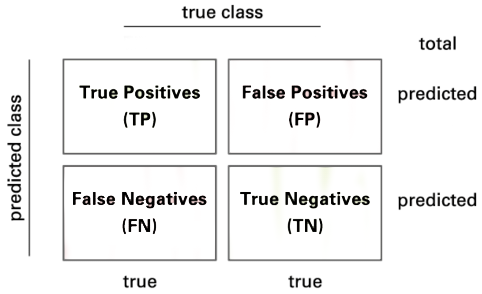
\includegraphics[width=0.7\linewidth]{Definitions/Confusion-matrix}
\caption{Confusion matrix.}\label{fig:confusion-matrix}
		\end{figure}\unskip
\begin{figure}[H]
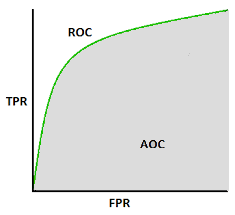
\includegraphics[width=.7\linewidth]{Definitions/AUC}
\caption{{Area} %MDPI: Please cite the figure in the text and ensure the first citation of each figure appears in numerical order. % H.K.D Citation provided
 under the curve.}\label{fig:AUC}
	\end{figure}
	
	The True Positive ({\textit{TP}}%MDPI: Please change the forward italics of the variables in the text and formulas to be consistent %H.K.D Italics word changed
) of all classes in this case is the main diagonal of the matrix $A$. The~following methods are used to calculate the False Positives ({\textit{FP}}%MDPI: Please change the forward italics of the variables in the text and formulas to be consistent %H.K.D Italics word changed
), False Negatives ({\textit{FN}}%MDPI: Please change the forward italics of the variables in the text and formulas to be consistent %H.K.D Italics word changed
), and~True Negatives ({\textit{TN}}%MDPI: Please change the forward italics of the variables in the text and formulas to be consistent %H.K.D Italics word changed
) of all classes:
	
	\begin{equation}
		\label{eqn:FP}
		FP = -TP + \sum_{k=1}^{i}A^i_k
	\end{equation}
	
	\begin{equation}
		\label{eqn:FN}
		FN = -TP + \sum_{k=1}^{j}A^j_k
	\end{equation}
	

\begin{adjustwidth}{-\extralength}{0cm}
%\centering %% If there is a figure in wide page, please release command \centering
	\begin{equation}
		\label{eqn:TN}
		TN_c = \sum_{i=1}^{C}\sum_{j=1}^{C}a_{ij} - \left[ \sum_{k=1}^{i}A^i_{i=c k} + \sum_{k=1}^{j}A^j_{j=c k} \right] + a_{i=c j=c} \implies TN = \begin{bmatrix}
TN_1 & TN_2 & \dots & TN_c
		\end{bmatrix}
	\end{equation}
\end{adjustwidth}
	
	{Then,} %MDPI: Please confirm should the no indentation be retained
	% H.K.D I think it would be better if there is no indentation but do not know to do it, could you help me remove it.
 the model is evaluated by the following metrics:
	
	\begin{equation}
		\label{eqn:sens}
		\text{\textit{Sensitivity (Sens)}} = \frac{TP}{TP + FN}
	\end{equation}
	
	\begin{equation}
		\label{eqn:spec}
		\text{\textit{Specificity (Spec)}} = \frac{TN}{TN + FP}
	\end{equation}
	
%	\change[H.K.D]{Sensitivity and Specificity mathematically describe the accuracy of a test that reports the presence or absence of a condition. Individuals for which the condition is satisfied are considered "positive" and those for which it is not considered "negative". Sensitivity or true positive rate refers to the probability of a positive test, conditioned on truly being positive while Specificity or true negative rate refers to the probability of a negative test, conditioned on truly being negative.}
	{{Sensitivity (Equation \mbox{\eqref{eqn:sens}}) and specificity (Equation \mbox{\eqref{eqn:spec}}) mathematically describe the accuracy of a test that identifies a condition's presence or absence. Sensitivity, also known as the true positive rate, is the likelihood that a test will result in a true positive, whereas specificity, also known as the true negative rate, is the likelihood that a test will result in a true negative.}}
	
	\begin{equation}
		\label{eqn:pre}
		\text{\textit{Precision}} = \frac{TP}{TP + FP}
	\end{equation}
	
	\begin{equation}
		\label{eqn:f1}
		\text{\textit{F1-score}} = \frac{2 \times TP}{2 \times TP + FP + FN + TN}\
	\end{equation}
	
	{Precision} %MDPI: Please confirm should the no indentation be retained
	% V.D.N confirmed
 (Equation \eqref{eqn:pre}) or positive predictive value (PPV) is the probability of a positive test conditioned on both truly being positive or negative. F1-score (Equation \eqref{eqn:f1}), on the other hand, refers to the harmonic mean of precision and recall, which means the higher the F1-score is, the higher both precision and recall are. Besides, the expected value of precision, F1-score, and recall are also applied because of the multi-class problem.
	
	\begin{equation}
		\label{eqn:acc}
		\text{\textit{Accuracy}} = \frac{TP + TN}{TP + FP + FN + TN}
	\end{equation}
	
	\begin{equation}
		\label{eqn:balacc}
		\text{\textit{Balanced Accuracy}} = \frac{\text{Sens} + \text{Spec}}{2}
	\end{equation}
	
	{The last} %MDPI: Please confirm should the no indentation be retained
	% V.D.N confirmed.
 metric is the $AUC$ {(as shown in Figure \mbox{\ref{fig:AUC}})} score standing for Area Under the Curve which is the Receiver Operating Curve (ROC) that indicates the probability of TP versus the probability of FP.  
	
	\subsection{Discussion} 
	\begin{comment}
		\begin{figure}[H]
\centering
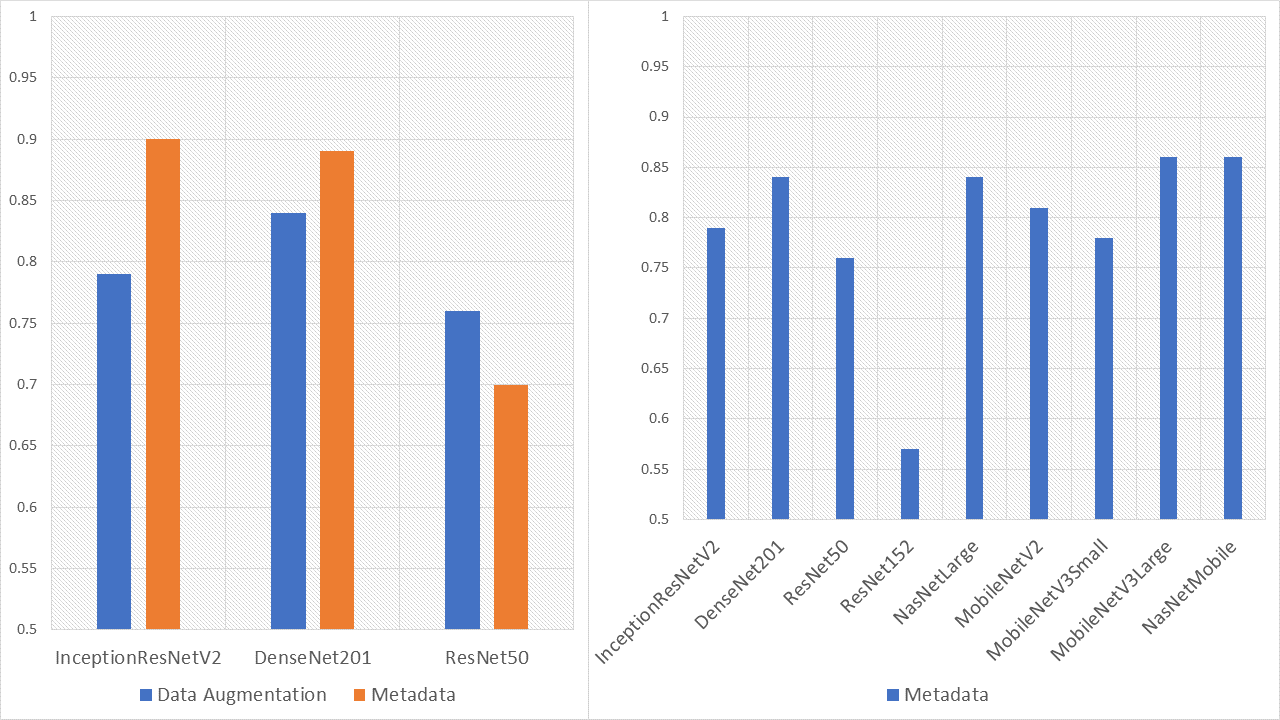
\includegraphics[width=1\linewidth]{Definitions/ACCALL}
\caption{Accuracy of all models trained in this research.}
\label{fig:accall}
		\end{figure}
	\end{comment}
	
	According to Table \ref{table:overall-acc}, it is clear that the model trained with metadata has a higher accuracy than the model trained with augmented data only. While InceptionResNetV2 and DenseNet201 trained with augmented data have an accuracy of $0.79$ and $0.84$, respectively, their training with metadata are $0.90$ and $0.89$, respectively. Furthermore, Resnet50 trained with metadata data has the accuracy that outperforms the Resnet50 trained with augmented data and is twice as high as ResNet152 trained with metadata. On the other hand, mobile models including MobileNetV2, MobileNetV3Large, and NasNetMobile, even though they have a much smaller number of parameters and depth than the other model, they have quite good accuracy scores of $0.81$, $0.86$ and $0.86$, respectively. 
	
	\begin{table}[H]
		\caption{Accuracy of all models. ACC stands for accuracy. AD stands for augmented data; this indicates that the model is trained with augmented data. MD stands for metadata, which indicates that the model is trained with metadata. The bold numbers highlight the highest performance.}
		\label{table:overall-acc}
		\setlength{\tabcolsep}{12.38mm}\begin{tabular}{ l  c  c  }
\toprule
\textbf{Model} & \textbf{ACC (AD)} & \textbf{ACC (MD)}\\ 
\midrule
InceptionResNetV2 & 0.79 & \textbf{{0.90} %MDPI: Please add an explanation for bold in the table footer. If the bold is unnecessary, please remove it. 
%H.K.D We have already explain it in the paragraph before the Table 5
}\\
\midrule
DenseNet201 & 0.84 & 0.89\\
\midrule
ResNet50 & 0.76 & 0.70\\
\midrule
ResNet152 & 0.81 & 0.57\\
\midrule
NasNetLarge & 0.56 & 0.84\\
\midrule
MobileNetV2 & 0.83 & 0.81\\
\midrule
MobileNetV3Small & 0.83 & 0.78\\
\midrule
MobileNetV3Large & 0.85 & \textbf{0.86}\\
\midrule
NasNetMobile & 0.84 & \textbf{0.86}\\
\bottomrule
		\end{tabular}
	\end{table}
	
	Moreover, the model trained with augmented data does not only have low accuracy but their F1-score and the recall also are imbalanced according to Figures \ref{fig:den f1}--\ref{fig:incep recall}. As a result, the augmented data model does not classify well in all class as InceptionResNetV2 trained on augmented data has an F1-score on class df and the akiec is just above $0.3$ and $0.4$, separately, while InceptionResNetV2 trained on metadata and the new weight loss can classify well in a balanced way according to the Figure \ref{fig:incep f1}. However, only DenseNet201, InceptionResNetV2, and NasNetLarge whose depths are equal to or larger than 400 have balanced the F1-scores on class. The others still face the imbalanced term. Since this data set is not balanced, therefore using augmented data can make the model more biased to the class which has a larger sample. Although using the metadata still leads to model biased, it does contribute to the improvement of the performance of the~model.
	
	\begin{figure}[H]
		\begin{minipage}{0.48\textwidth}
\centering
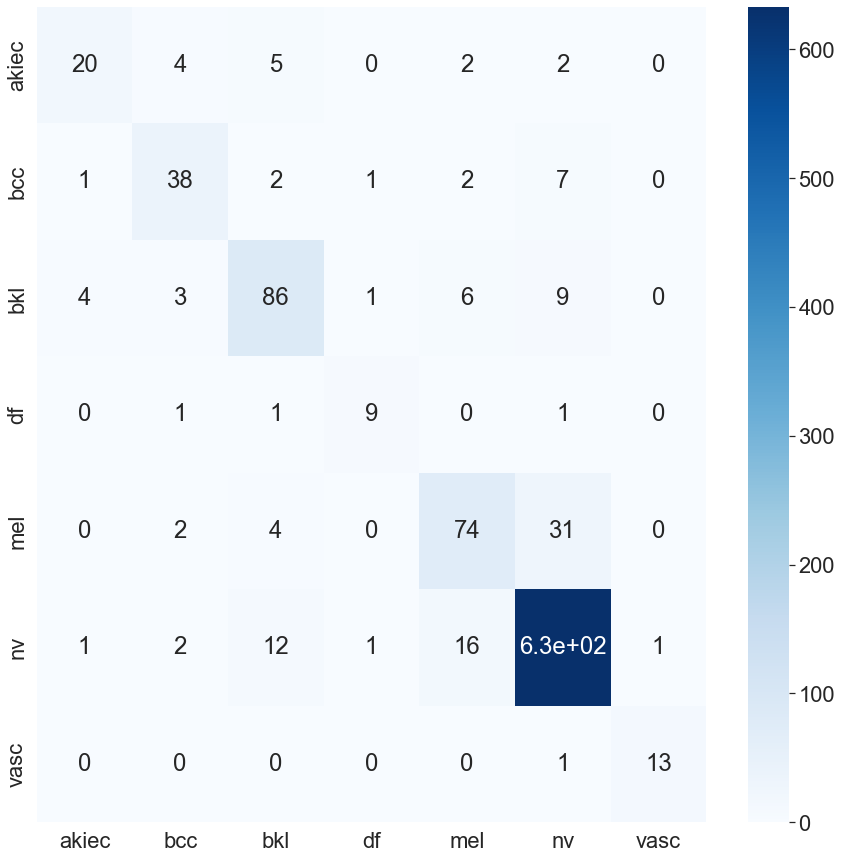
\includegraphics[width=1.3\linewidth]{Definitions/CM/dn201cm}
		\end{minipage}
\caption{{DenseNet201} %MDPI: Please cite the figure in the text and ensure the first citation of each figure appears in numerical order.
	% H.K.D Citation Provided
 confusion matrix.}\label{fig:densenet201cm}
		\end{figure}\unskip
		
		\begin{figure}[H]
		\begin{minipage}{0.48\textwidth}
\centering
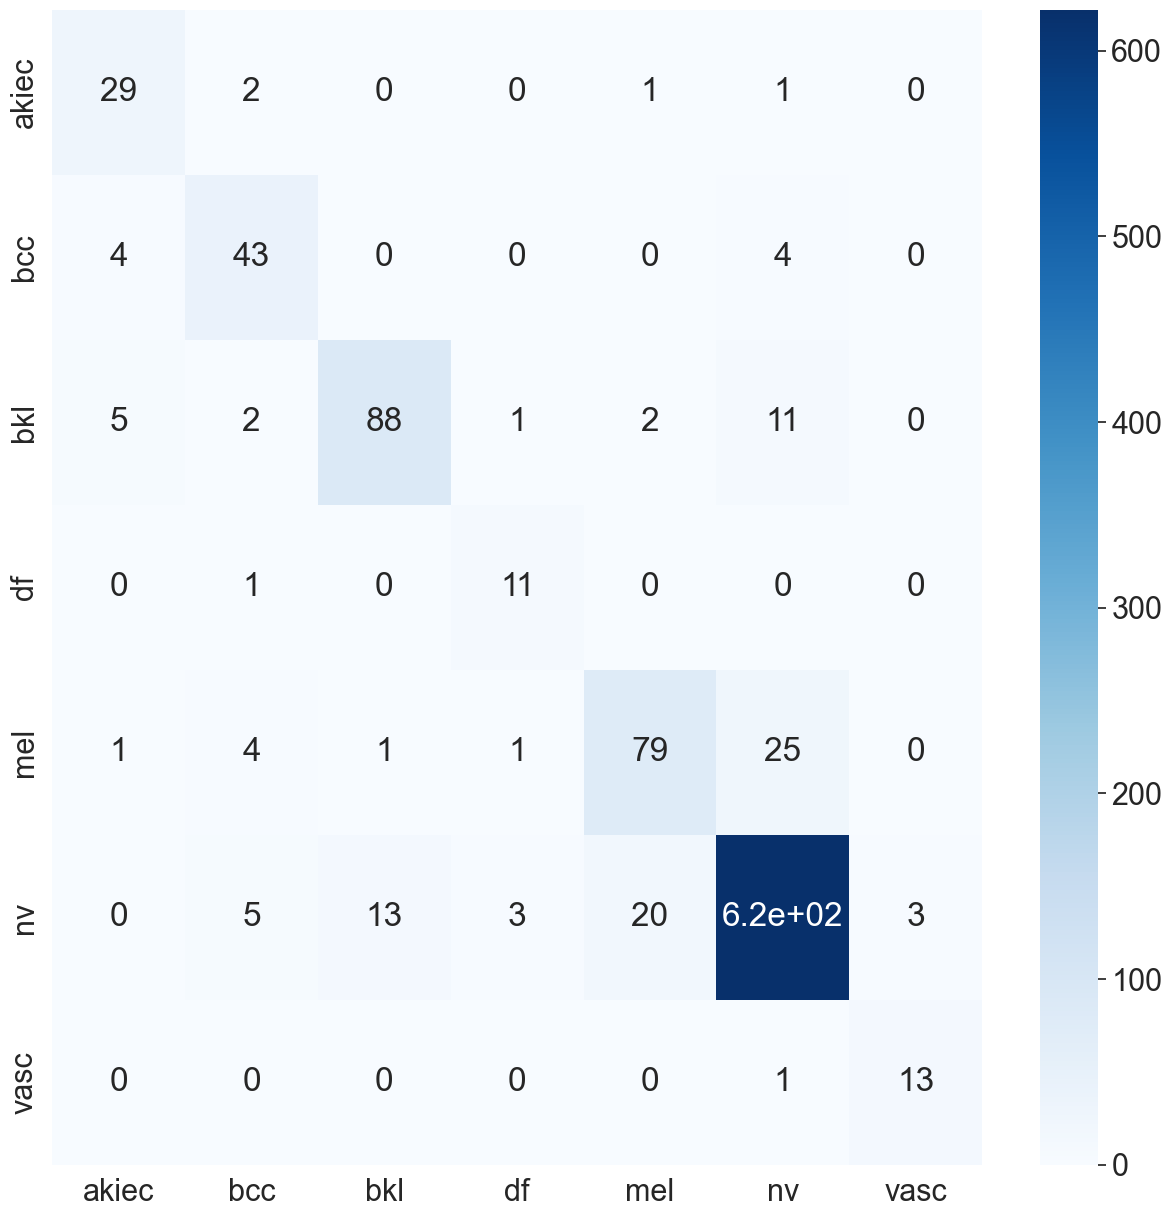
\includegraphics[width=1.3\linewidth]{Definitions/CM/irv2cm}
		\end{minipage}
\caption{{InceptionResNetV2} %MDPI: Please cite the figure in the text and ensure the first citation of each figure appears in numerical order.
% H.K.D Citation Provided
 confusion matrix.}\label{fig:irv2cm}
	\end{figure}
	
	\begin{figure}[H]
		\centering
		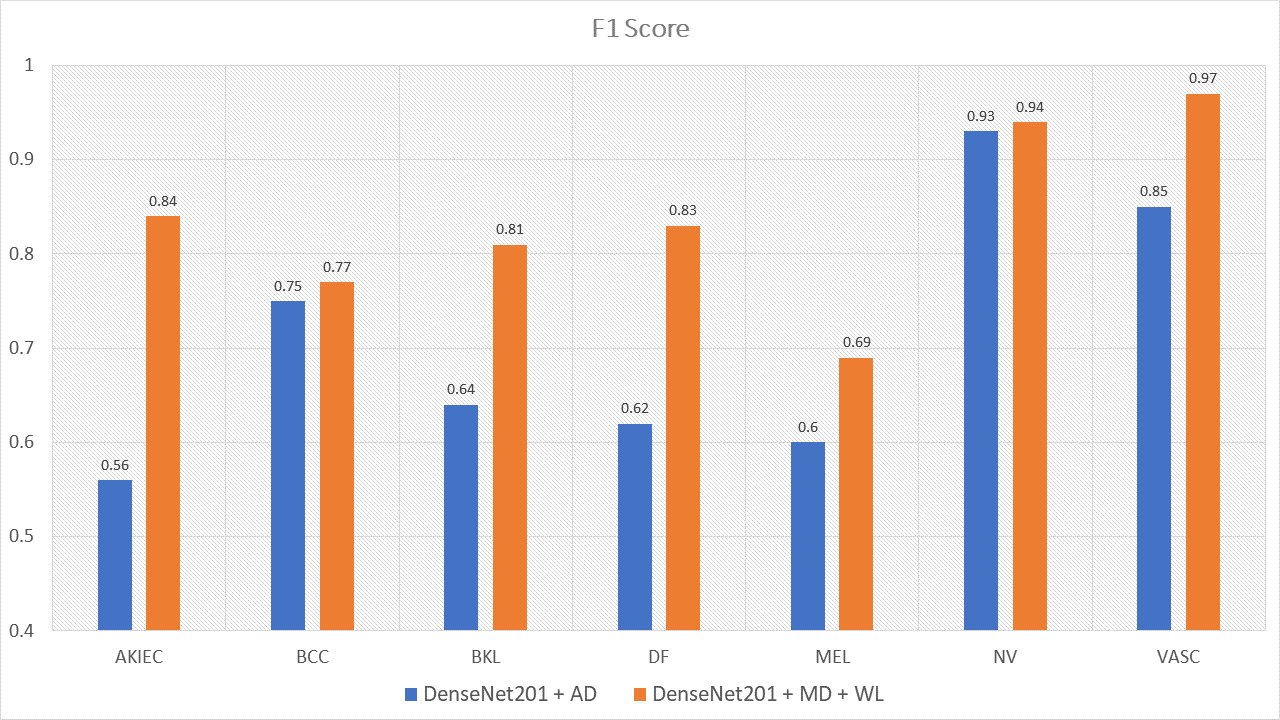
\includegraphics[width=1\linewidth]{Definitions/den f1.PNG}
		\caption{The comparison between F1-scores of DenseNet201 trained with augmented data and the one trained with metadata and weight loss.}
		\label{fig:den f1}
	\end{figure}\unskip
	\begin{figure}[H]
		\centering
		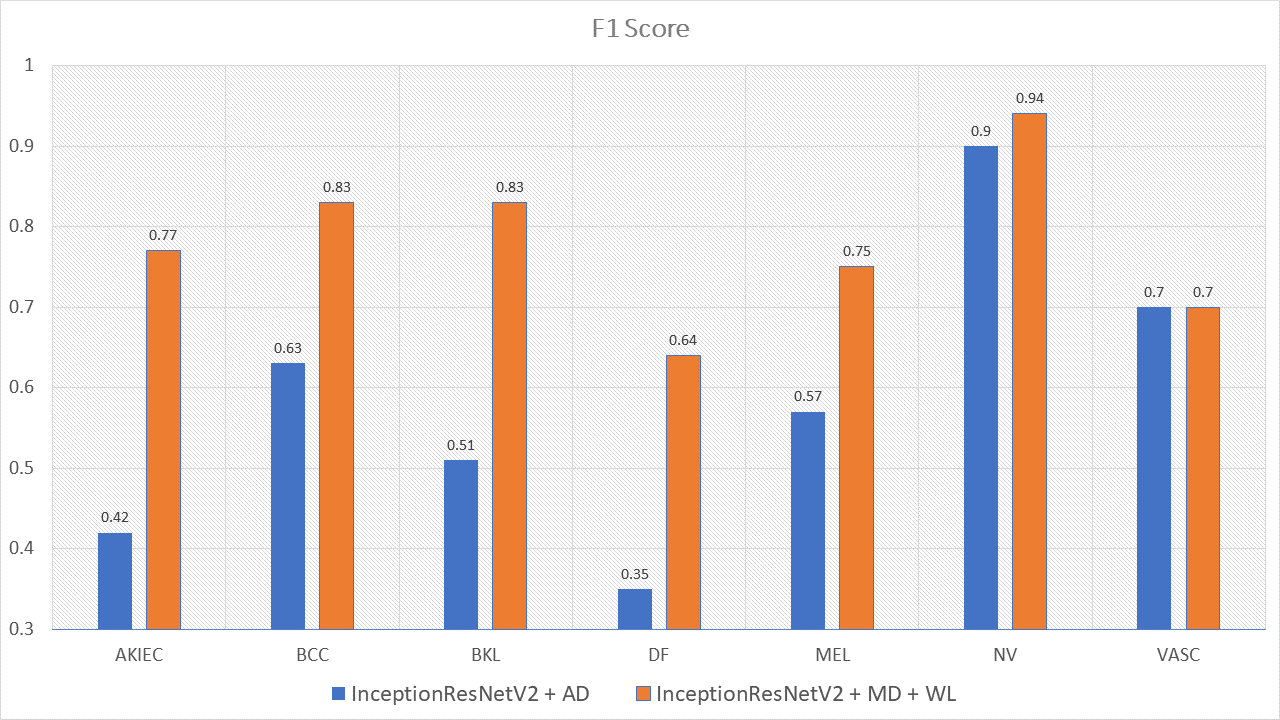
\includegraphics[width=1\linewidth]{Definitions/in f1.PNG}
		\caption{The comparison between F1-scores of InceptionResNetV2 trained with augmented data and the one trained with metadata and weight loss.}
		\label{fig:incep f1}
	\end{figure}
	
\textls[-15]{	This problem is also true with the recall according to Figures \ref{fig:den recall} and \ref{fig:incep recall}. DenseNet201 and InceptionResNetV2, trained with augmented data have expected recall values of $0.56$ and $0.69$, respectively, while the combination of DenseNet201, Metadata, and the new weight loss function achieve the expected value of recall: $0.82$. Therefore, metadata do improve the model performance by reducing the amount of data needed for achieving higher results. On the other hand, the reason why the model becomes much more balanced is the weighted loss function. Weight loss function has the ability to solve the imbalanced class samples by adding a weight related to the number of samples in each class. DenseNet201 and InceptionResNetV2 trained with the new weighted loss function have recall in akiec of $0.85$ and $0.82$, respectively, as opposed to their training in akiec without weighted loss function: $0.65$ and $0.37$. }
	
	\begin{figure}[H]
		\centering
		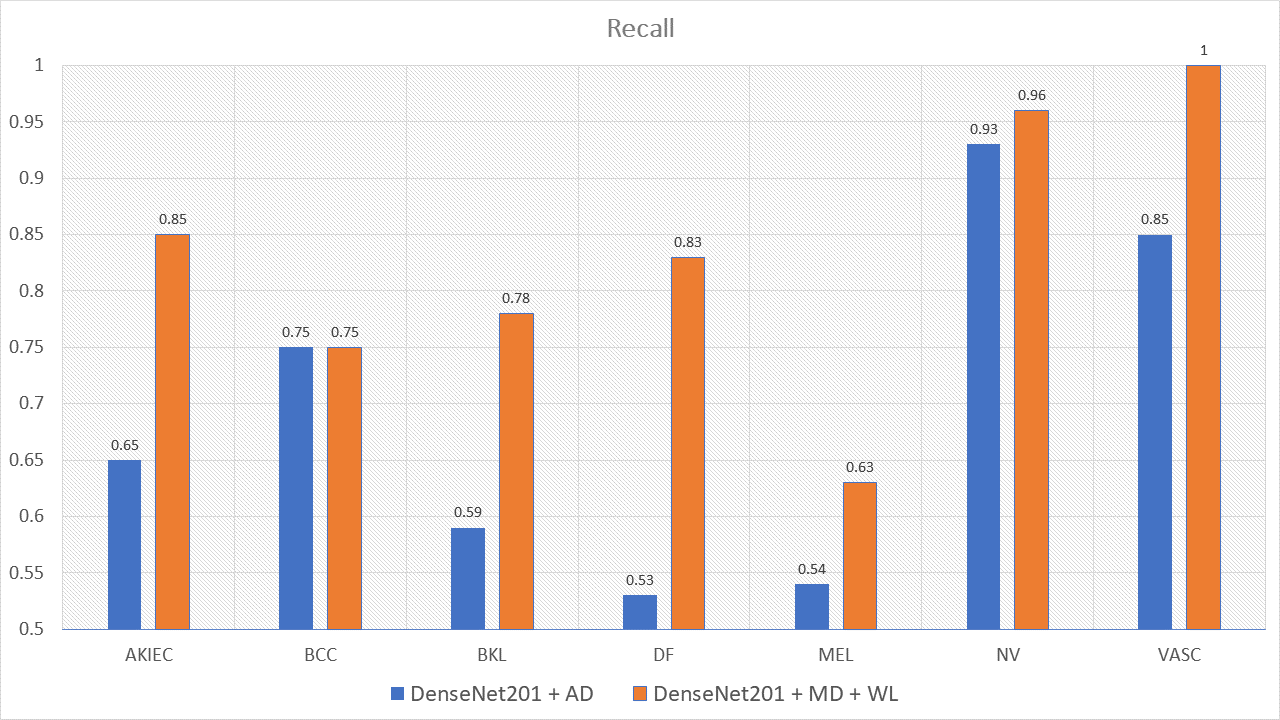
\includegraphics[width=1\linewidth]{Definitions/den re.PNG}
		\caption{The comparison between recall of DenseNet201 trained with augmented data and the one trained with metadata and weight loss.}
		\label{fig:den recall}
	\end{figure}\unskip
	
	\begin{figure}[H]
		\centering
		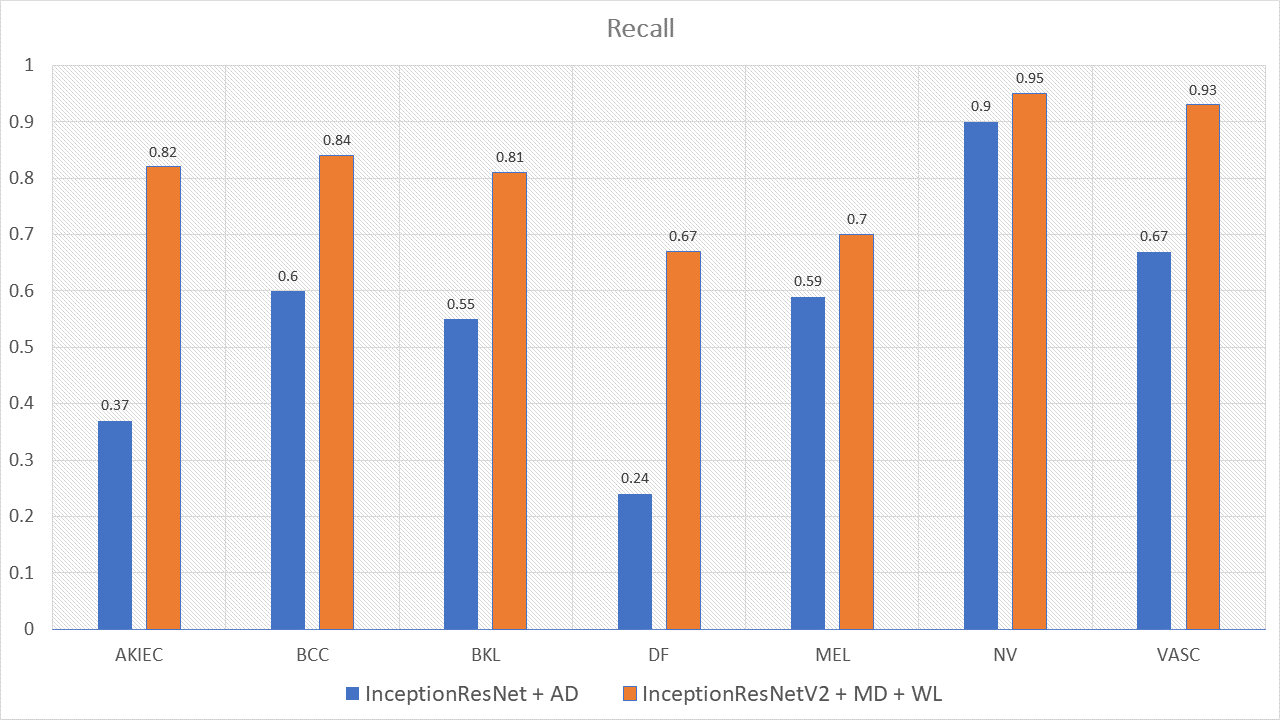
\includegraphics[width=1\linewidth]{Definitions/in re.PNG}
		\caption{Comparison between recall of InceptionResNetV2 trained with augmented data and the one trained with metadata and weight loss.}
		\label{fig:incep recall}
	\end{figure}
	
	Another interesting point found during the experiment is that MobileNetV2, MobileNetV3, and NasNetMobile have a small number of parameters and depth, but they have relatively good performance. MobileV3large, MobileV3Small, NasNetLarge and NasNetMobile outperform others on classifying class df with the recall of $0.92$, $1$, $0.92$ and  $0.92$, respectively, according to the Table \ref{appendix-table:mobile-performance}. It is obvious that MobileNetV3Large and NasNetMobile are the two best performance models. Nevertheless, MobileNetV3Large has fewer number of parameters and depth than NasNetMobile.

	Table \ref{table:optimized-performance-mobile-model} shows that the MobileNetV3Large, although the number of parameters is much smaller than that of DenseNet201. InceptionResNetV2, achieves an accuracy nearly to the others. In detail, MobileNetV3Large whose number of parameters has 5.5 million parameters, which is four and ten times less than DenseNet201 and InceptionResNetV2, respectively. The depth of MobileNetV3Large, on the other hand, is four times less than DenseNet201, InceptionResNetV2 which are 118 hidden layers as opposed to the 402 and 449 values of DenseNet201 and InceptionResNetV2, separately. Although, MobileNetV3Larege only achieves an accuracy of 0.86, the time needed for prediction is 10 and 30 times less than the other opponents. Since MobileNetV3Large needs a harder process of parameter hyper-tuning to achieve a better result, this is also the future target of this research.
	
	\begin{table}[H]
		\caption{%\change[H.K.D]{Performance Comparison between MobileNetV3Large and DenseNet201, InceptionResNetV2} %V.D.N We have already changed the caption of Figure 6
		{Comparison between MobileNetV3Large with DenseNet201 and InceptionResNetV2.}}
		\label{table:optimized-performance-mobile-model}

\begin{adjustwidth}{-\extralength}{0cm}
\centering %% If there is a figure in wide page, please release command \centering
		\setlength{\tabcolsep}{6.6mm}\begin{tabular}{ l  c  c  c }
\toprule
\textbf{Model} & \textbf{MobileNetV3Large} & \textbf{DenseNet201} & \textbf{InceptionResnetV2}\\
\midrule
No. Trainable Parameters & \textbf{{5,490,039} %MDPI: Please add an explanation for bold in the table footer. If the bold is unnecessary, please remove it. The following highlights are the same.
} & 17,382,935 & 47,599,671\\
\midrule
Depth & \textbf{118} & 402 & 449\\
\midrule
Accuracy & 0.86 & 0.89 & 0.90\\
\midrule
Training Time (seconds/epoch) & 116 & 1000 & 3500\\
\midrule
Infer Time (seconds) & \textbf{0.13} & 1.16 & 4.08 \\
\bottomrule
		\end{tabular}
\end{adjustwidth}
	\end{table}
	Table \ref{table:overall-auc} shows the AUC of the three models—InceptionResNetV2, Densenet201, and ResNet50—which are trained with only augmented data or metadata. It is transparent that the InceptionResNetV2 and DenseNet201 have higher AUC trained with metadata: both 0.99 as opposed to 0.972 and 0.93, respectively. ResNet50 trained with augmented data, on the other hand, has a higher AUC of 0.95 as compared to 0.93 of ResNet50 trained with metadata. Overall, InceptionResNetV2 trained with metadata reaches the peak with an AUC of 0.974. The InceptionResNetV2 trained with metadata is also compared with the others to find out the best models trained. According to Figure {\mbox{\ref{fig:densenet201cm}, \ref{fig:irv2cm}, and \ref{fig:densevsirv2}}} the InceptionResNetV2 still hit the peak AUC of 0.99. In contrast, ResNet152 otherwise is the worst model with the AUC of 0.87. Other models, on the other hand, have the approximately the same AUC. 
	
	\begin{table}[H]
			\caption{AUCs of all models. AD stands for augmented data, this indicates that the model is trained with augmented data. MD stands for metadata, which indicates that the model is trained with metadata. Bold numbers highlight the highest performance}
		\label{table:overall-auc}
	\setlength{\tabcolsep}{12.3mm}\begin{tabular}{ l  c  c  }
\toprule
\textbf{Model} & \textbf{AUC (AD)} & \textbf{AUC (MD)}\\ 
\midrule
InceptionResNetV2 & 0.971 & \textbf{{0.99} %MDPI: Please add an explanation for bold in the table footer. If the bold is unnecessary, please remove it. The following highlights are the same.
%H.K.D We have already added the explaination in the paragraph before the Table 7
}\\
\midrule
DenseNet201 & 0.93 & \textbf{0.99}\\
\midrule
ResNet50 & 0.95 & 0.93 \\
\midrule
ResNet152 & 0.97 & 0.87\\
\midrule
NasNetLarge & 0.74 & 0.96\\
\midrule
MobileNetV2 & 0.95 & \textbf{0.97}\\
\midrule
MobileNetV3Small & 0.67 & 0.96\\
\midrule
MobileNetV3Large & 0.96 & \textbf{0.97}\\
\midrule
NasNetMobile & 0.96 & \textbf{0.97}\\
\bottomrule
		\end{tabular}
	\end{table}\unskip
	
	\begin{figure}[H]
		\centering
		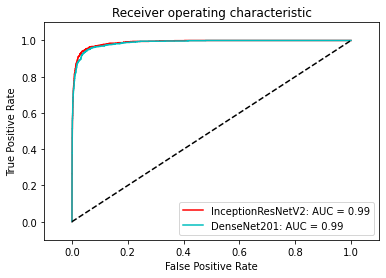
\includegraphics[width=1\linewidth]{Definitions/ROC/denvsirv2}
		\caption{ROC of DenseNet201 and InceptionResNetV2.}\label{fig:densevsirv2}
	\end{figure}
			

	In addition to the comparison between the original weight loss calculated by the sample percentage of each class model and the new weight loss-based model, it is also conducted on the three best-performing models including InceptionResNetV2, DenseNet201, and MobileNetV3. After the experiment, it is found out that the new weight loss function does not only contribute to the model to overcome the data imbalance problem but it also makes the accuracy increase. The performance of models is described in Table \ref{table:loss-comparision}.
	
	According to {Tables} %MDPI: there is no table:densenet201auc in the tex, please check and revise.
	% H.K.D We have removed the unnecessary part
	\ref{table:loss-comparision}, the InceptionResNetV2 is found to be the best model trained. Furthermore, the InceptionResNetV2 is compared with the other state of the art researched models. According to Table \ref{table:comparative-analysis}, there are six researchers that use the same data set: HAM10000 but they have  different approaches. These models used in that research are also SOTA models sorted in ascending order. The table shows that the accuracy of the combination of InceptionResNetV2 with Soft-Attention, metadata, and weight loss in this research is less than that of InceptionResNetV2 with Soft-Attention and augmented data: 0.90 compared to 0.93 respectively. However, since Soumyyak~et~al. uses data augmentation for all class of an imbalanced data set, the F1-score and recall are much lower. This is because the model in that research can only classify well on NV and VASC classes, which have the highest number of samples. On the other hand, the InceptionResNetV2 in this research also outperforms the other models according to five indicators: accuracy, precision, F1-score, recall, and AUC. 
	\begin{table}[H]
			\caption{Loss-based model accuracy comparison.}
		\label{table:loss-comparision}
	\setlength{\tabcolsep}{2.8mm}\begin{tabular}{ l  c  c  c }
\toprule
\textbf{Model} & \textbf{No Weight} & \textbf{Original Loss Accuracy} & \textbf{New Loss Accuracy}\\
\midrule
InceptionResNetV2 & 0.74 & 0.79 & 0.90\\
DenseNet201 & 0.81 & 0.84 & 0.89\\
MobileNetV3Large & 0.79 & 0.80 & 0.86\\
\bottomrule
		\end{tabular}
	\end{table} 
\unskip

	
	
	\begin{table}[H]
		\caption{Comparative Analysis. Bold numbers highlight the highest performance.}
		\label{table:comparative-analysis}
				\setlength{\tabcolsep}{1.6mm}\begin{tabular}{ p{5cm}  c  c  c  c  c }
\toprule
\textbf{Approach} & \textbf{Accuracy} & \textbf{Precision} & \textbf{F1-score} & \textbf{Recall} & \textbf{AUC}\\
\midrule
InceptionResNetV2~\cite{03358} & 0.93 & 0.89 & 0.75 & 0.71 & 0.97\\
\midrule
\cite{03798} & - & 0.88 & 0.77 & 0.74 & - \\
\midrule
\cite{09418} & 0.88 & - & - & - & - \\
\midrule
\cite{01284} & 0.86 & - & - & - & - \\
\midrule
GradCam and Kernel SHAP~\cite{06612} & 0.88 & - & - & - & - \\
\midrule
Student and Teacher~\cite{03225} & 0.85 & 0.76 & 0.76 & - & - \\
\midrule
Proposed Method & 0.9	& 0.86 & {\textbf{0.86}} & {\textbf{0.81}} & {\textbf{0.99}}%MDPI: Please confirm if the bold should be retained. If not necessary, please remove. %V.D.N We confirmed to continue to use bold numbers.
\\
\bottomrule
		\end{tabular}
	\end{table} 

However, there are still some drawbacks of the model: the InceptionResNetV2 cannot well classify the melanoma and the nevus. According to Figure \ref{fig:nevusVSmela} the model sometime classifies the black nevus as the melanoma because of the same color between them. However, this problem is not true for the hard black or big melanoma or the red black nevus. Some future approaches that can be proposed would be to change the type of color to the other to fix the same color problem.    
	
	\begin{figure}[H]
		\centering
		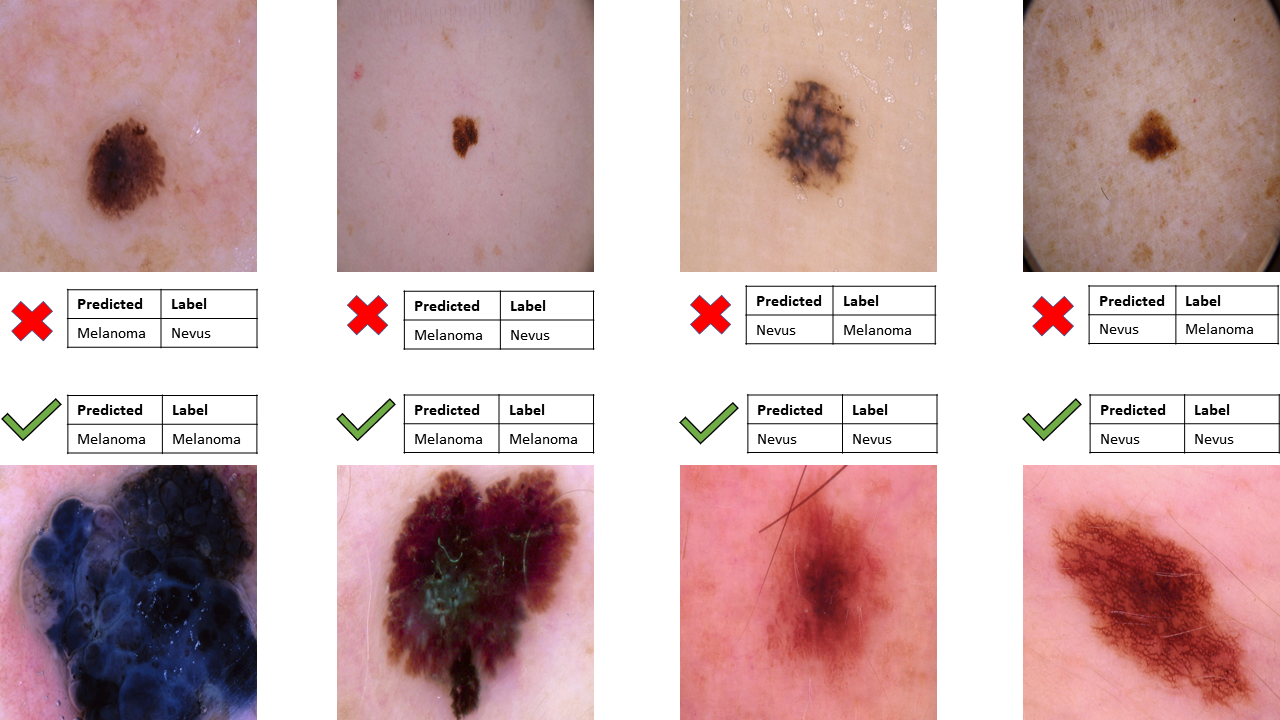
\includegraphics[width=0.9\linewidth]{Definitions/img_class_nevus_mela}
		\caption{Model ability to classify melanoma and nevus.}
		\label{fig:nevusVSmela}
	\end{figure}
	
	\section{Conclusions}
	In this work, we proposed a model formed by a combination of one backbone model and Soft-Attention. Moreover, the model takes two inputs, including image data and metadata. A new weight loss function is applied to figure out the data imbalance problem. Finally, the combination of InceptionResNetV2, Soft-Attention, and metadata is the best model with an accuracy of 0.9. Although the accuracy and the precision of the model are not the highest, the F1-score, recall, and AUC of 0.86, 0.81, and 0.975, respectively are the highest and the most balanced indicators. Therefore, InceptionResnetV2 can classify well in all classes including low-samples classes. Otherwise, during the experiment, the combination of MobileNetV3, Soft-Attention, and metadata achieves an accuracy of 0.86 that is nearly the same as InceptionResNetV2, although with fewer number parameters and depth. Therefore the infer time is much less than that of  InceptionResNetV2. This result opens the door to constructing a great performance model that can be applied to mobile and IoT devices. {As a result, the proposed method and others still face the problem of badly distinguishing between melanoma and black nevus because in some cases, the melanoma and the nevus image have the same lesion size and color.}
	\vspace{6pt} 
	
	%%%%%%%%%%%%%%%%%%%%%%%%%%%%%%%%%%%%%%%%%%
	%% optional
	%\supplementary{The following supporting information can be downloaded at:  \linksupplementary{s1}, Figure S1: title; Table S1: title; Video S1: title.}
	
	% Only for the journal Methods and Protocols:
	% If you wish to submit a video article, please do so with any other supplementary material.
	% \supplementary{The following supporting information can be downloaded at: \linksupplementary{s1}, Figure S1: title; Table S1: title; Video S1: title. A supporting video article is available at doi: link.}
	
	%%%%%%%%%%%%%%%%%%%%%%%%%%%%%%%%%%%%%%%%%%
	\authorcontributions{Conceptualization, V.D.N. and H.K.D.; methodology, V.D.N. and H.K.D.; software, H.K.D.; validation, V.D.N., N.D.B. and H.K.D.; formal analysis, V.D.N. and H.K.D.; investigation, V.D.N., N.D.B. and H.K.D.; resources, V.D.N.; data curation, H.K.D.; writing---original draft preparation, H.K.D.; writing---review and editing, V.D.N. and N.D.B.; visualization, H.K.D.; supervision, V.D.N. and N.D.B.; project administration, V.D.N. All authors have read and agreed to the published version of the manuscript.}
	
	\funding{This research received no external funding.}
	
	\institutionalreview{Not applicable.}
	
	\informedconsent{Not applicable.}
	
	\dataavailability{\textls[-15]{The code and the data analysis report can be found here:} \url{https://github.com/KhoiDOO/Skin-Disease-Detection-HAM100000.git}  ({accessed on 29 August 2022}%MDPI: Please add the access date (Format: Date Month Year) that earlier than Received date. e.g., (accessed on 29 August 2022).
	% H.K.D Access on Date has been provided
).} 
	\acknowledgments{We thank Vingroup innovation Foundation (VINIF) project code \\VINIF.2021.DA00192 for providing computational resources for the work} %V.D.N We have provided the acknowledgement.
	
	\conflictsofinterest{The authors declare no conflict of interest.} 
	
	%%%%%%%%%%%%%%%%%%%%%%%%%%%%%%%%%%%%%%%%%%
	%% Optional
%	\sampleavailability{}
	
	%% Only for journal Encyclopedia
	%\entrylink{The Link to this entry published on the encyclopedia platform.}
	
	\abbreviations{Abbreviations}{
		The following abbreviations are used in this manuscript:\\
		
		\noindent 
		\begin{tabular}{@{}ll}
CAD & Computer-aided diagnosis\\
AI & Artificial Intelligence\\
AKIEC & Actinic keratoses and intraepithelial carcinoma or Bowen's disease\\
BCC & Basal Cell Carcinoma\\
BKL & Benign Keratosis-like Lesions\\
DF & Dermatofibroma\\
MEL & Melanoma\\
NV & Melanocytic Nevi\\
VASC & Vascular Lesions\\
HISTO & Histopathology\\
FOLLOWUP & Follow-up examination\\
CONSENSUS & Expert Consensus\\
CONFOCAL & Confocal Microscopy\\
RGB & Red Green Blue\\
BGR & Blue Green Red\\
TP & True Positives\\
FN & False Negatives\\
TN & True Negatives\\
FP & False Positives\\
Sens & Sensitivity\\
Spec & Specificity\\
AUC & Area Under the Curve\\
ROC & Receiver Operating Curve\\
		\end{tabular}
	}
	
	%%%%%%%%%%%%%%%%%%%%%%%%%%%%%%%%%%%%%%%%%%
	%% Optional
	
	\appendixtitles{yes} 
	\appendixstart
	\appendix
\startlandscape

\begin{adjustwidth}{+\extralength}{0cm}
%\centering %% If there is a figure in wide page, please release command \centering
	\section[\appendixname~\thesection]{Detailed Model Structure}
	
	\begin{table}[H]
			\caption{{Detailed structure} %MDPI: 1. We revised the "x" into a multiplication sign ("\times" U+00D7). Please confirm. 2. Please confirm if the vertical line is necessary, if not, please remove it.
			% H.K.D Incredibly beautiful table
 of models except for mobile models. SA stands for Soft-Attention, SA Module denotes whether that model uses the Soft-Attention module. GAP stands for Global Average Pooling. FC stands for Fully Connected Layer.\label{appendix-table:detailed structure model}}
%\newcolumntype{C}{>{\centering\arraybackslash}X}
\begin{tabularx}{\textwidth}{p{2.2cm}  p{2.2cm}  p{2.2cm}  p{2.6cm}  p{2.2cm}  p{2.2cm}  p{2.2cm}  p{2.2cm}  p{2.4cm}  p{2.6cm}}
	\toprule
	\textbf{DenseNet-201} & \textbf{DenseNet-201 + SA} & \textbf{Inception-ResNetV2} & \textbf{Inception-ResNetV2 +~SA} & \textbf{ResNet-50} & \textbf{ResNet-50 +~SA} & \textbf{ResNet-152} & \textbf{ResNet-152 +~SA} & \textbf{NasNet-Large} & \textbf{NasNet-Large +~SA}\\
	\midrule
	Conv2D $7 \times 7$ & Conv2D $7 \times 7$ & STEM& STEM& Conv2D $7 \times 7$& Conv2D $7 \times 7$& Conv2D $7 \times 7$& Conv2D $7 \times 7$& Conv2D $3 \times 3$& Conv2D $3 \times 3$\\ \midrule
	Pooling $3 \times 3$ & Pooling $3 \times 3$ & & & Pooling $3 \times 3$& Pooling  $3 \times 3$& Pooling  $3 \times 3$& Pooling  $3 \times 3$& Pooling& Pooling\\ \midrule		
	DenseBlock $\times$~6 & DenseBlock $\times$~6 & Inception ResNet A $\times$~10& Inception ResNet A $\times$~10& Residual Block $\times$~3& Residual Block $\times$~3& Residual Block $\times$~3& Residual Block $\times$~3& Reduction Cell $\times$~2& Reduction Cell $\times$~2\\  \midrule
	Conv2D $1 \times 1$ & Conv2D $1 \times 1$ & Reduction A & Reduction A & & & & & Normal Cell $\times$~N& Normal Cell $\times$~N\\	\midrule
	Average pool $2 \times 2$ & Average pool $2 \times 2$ & & & & & & & & \\ \midrule
	DenseBlock $\times$~12 & DenseBlock $\times$~12 & Inception ResNet B $\times$~20& Inception ResNet B $\times$~20& Residual Block $\times$~4& Residual Block $\times$~4& Residual Block $\times$~8& Residual Block $\times$~8& Reduction Cell& Reduction Cell\\ \midrule
	Conv2D $1 \times 1$ & Conv2D $1 \times 1$ & Reduction B & Reduction B & & & & & Normal Cell $\times$~N& Normal Cell $\times$ N\\\midrule
	Average pool $2 \times 2$ & Average pool $2 \times 2$ & & & & & & & & \\ \midrule
	DenseBlock $\times$ 48 & DenseBlock $\times$~12 & Inception ResNet C $\times$~5& Inception ResNet C $\times$~5& Residual Block $\times$~6& Residual Block $\times$ 6& Residual Block $\times$~36& Residual Block $\times$~36& Reduction Cell& Reduction Cell\\ \midrule
	Conv2D $1 \times 1$ & Conv2D $1 \times 1$ & & & & & & & Normal Cell $\times$~N& Normal Cell $\times$~N-2\\\midrule
	Average pool $2 \times 2$ & Average pool $2 \times 2$ & & & & & & & & \\ \midrule
	DenseBlock $\times$~29 & DenseBlock $\times$~29 & & & Residual Block $\times$~3& & Residual Block $\times$~3& & & \\ \midrule
	DenseBlock $\times$ 3 & \textbf{\hl{SA Module} %MDPI: Please confirm if the bold should be retained. % H.K.D It should be retained
} & & \textbf{SA Module}& & \textbf{SA Module}& & \textbf{SA Module}& & \textbf{SA Module}\\	\midrule
	GAP $7 \times 7$ & & Average pool& & GAP $7 \times 7$& & GAP $7 \times 7$& & & \\\midrule
	FC 1000D & & Dropout (0.8)& & FC 1000D& & FC 1000D& & & \\ \midrule
	SoftMax & SoftMax & SoftMax& SoftMax& SoftMax& SoftMax& SoftMax& SoftMax& SoftMax& SoftMax\\ 
	\bottomrule
\end{tabularx}
	\end{table}
	
	\section[\appendixname~\thesection]{Detailed Mobile-based Model Structure}
	
	\begin{table}[H]
		\caption{{Detailed} structure of mobile-based models. SA stands for Soft-Attention, SA Module denotes whether that model uses the Soft-Attention module. SE which stands for Squeeze-And-Excite, and it shows whether that block has Squeeze-And-Excite. \label{appendix-table:detailed mobile model structure}}%MDPI: We remove the vertical line, please confirm.
		% The most fantastic and spectacular table in the world
%\newcolumntype{C}{>{\centering\arraybackslash}X}
\begin{tabularx}{\textwidth}{p{3cm}  p{3cm}  p{4.2cm}  p{3cm}  p{3cm}  p{3cm}  p{2.3cm}  p{2.3cm}}
	\toprule
	\textbf{MobileNetV2} & \textbf{MobileNetV2 + SA} & \textbf{MobileNetV3 Small} & \textbf{MobileNetV3 Small + SA} & \textbf{MobileNetV3 Large} & \textbf{MobileNetV3 Large + SA} & \textbf{NasNet Mobile} & \textbf{NasNetMobile + SA}\\
	\midrule
	Conv2D & Conv2D& Conv2D $3 \times 3$& Conv2D $3 \times 3$& Conv2D $3 \times 3$& Conv2D $3 \times 3$ & Normal Cell & Normal Cell\\	\midrule		
	bottleneck & bottleneck & bottleneck $3 \times 3$ SE& bottleneck $3 \times 3$ SE& bottleneck $3 \times 3$ 3 repeated& bottleneck $3 \times 3$ 3 repeated& Reduction Cell& Reduction Cell\\ \midrule		
	bottleneck 2 repeated& bottleneck 2 repeated& bottleneck $3 \times 3$& bottleneck $3 \times 3$& bottleneck $5 \times 5$ SE 3 repeated& bottleneck $5 \times 5$ SE 3 repeated & Normal Cell & Normal Cell\\ \midrule	
	bottleneck 3 repeated& bottleneck 3 repeated& bottleneck $5 \times 5$ SE 8 repeated& bottleneck $5 \times 5$ SE 8 repeated& bottleneck $3 \times 3$ 4 repeated& bottleneck $3 \times 3$ 4 repeated& Reduction Cell & Reduction Cell\\ \midrule	
	bottleneck 4 repeated& bottleneck 4 repeated& & & bottleneck $3 \times 3$ SE 2 repeated& bottleneck $3 \times 3$ SE 2 repeated & Normal Cell\\ \midrule	
	bottleneck 3 repeated& bottleneck 3 repeated& & & bottleneck $5 \times 5$ SE 3 repeated& bottleneck $5 \times 5$ SE 3 repeated& \\ \midrule	
	bottleneck 3 repeated& bottleneck & & & & & \\ \midrule	
	bottleneck & & & & & & \\ \midrule
	Conv2D $1 \times 1$ & & Conv2D $1 \times 1$ SE & Conv2D $1 \times 1$ SE& Conv2D $1 \times 1$& Conv2D $1 \times 1$ & & \\ \midrule
	AP $7 \times 7$ & & Pool $7 \times 7$& Pool $7 \times 7$& Pool $7 \times 7$& Pool $7 \times 7$& &\\ \midrule
	Conv2D $1 \times 1$ & \textbf{SA Module}& Conv2D $1 \times 1$ 2 repeated& \textbf{SA Module}& Conv2D $1 \times 1$ 2 repeated& \textbf{SA Module}& &\textbf{SA Module}\\ \midrule
	Softmax & Softmax& Softmax& Softmax& Softmax& Softmax& Softmax & Softmax\\ 
	\bottomrule
\end{tabularx}
	\end{table}

\end{adjustwidth}	\finishlandscape
	%%%%%%%%%%%%%%%%%%%%%%%%%%%%%%%%%%%%%%%%%%
		
		\section[\appendixname~\thesection]{Detailed Model Performance}
		\subsection[\appendixname~\thesection]{F1-Score Model Performance}
		\begin{table}[H]
\caption{{F1-score%MDPI: Please confirm if the vertical line is necessary, if not, please remove it. 
% H.K.D beautiful no vertical line
} of each class: akiec, bcc, bkl, df, mel, nv and vasc, which are denoted in the abbreviations. The last column shows the expected value of the F1-score from each model. All models in the first column are the models trained in this research. The term “with Augmented Data” means that model is trained with data augmenting during the training, there is no metadata or weight loss contribution. The term “with Metadata and WeightLoss” means that the model is trained with metadata including age, gender, localization, and the weight loss function, there is no augmented data contribution. {Besides the bold number highlights achievement of the research}}
\label{appendix-table:F1-score-summary}

\begin{adjustwidth}{-\extralength}{0cm}
%\centering %% If there is a figure in wide page, please release command \centering
\centering
\begin{tabular}{p{9cm}  p{0.8cm}  p{0.8cm}  p{0.6cm}  p{0.6cm}  p{0.6cm}  p{0.6cm}  p{0.8cm}  p{0.9cm}} 
	\toprule
	\textbf{Model} & \textbf{akiec} & \textbf{bcc} & \textbf{bkl} & \textbf{df} & \textbf{mel} & \textbf{nv} & \textbf{vasc} & \textbf{Mean} \\
	\midrule
	DenseNet201 with Augmented Data & 0.56 & 0.75 & 0.64 & 0.62 & 0.60 & 0.93 & 0.85 & 0.70 \\ 
	\midrule
	InceptionResNetV2 with Augmented Data & 0.42 &	0.63 & 0.51 & 0.35 & 0.57 & 0.9 & 0.7 & 0.58\\
	\midrule
	Resnet50 with Augmented Data & 0.39 & 0.59 & 0.42 & 0.6 & 0.42 & 0.88 & 0.79 & 0.58\\
	\midrule 	
	VGG16 with Augmented Data & 0.35 & 0.62 & 0.42 & 0.32 & 0.47 & 0.89 & 0.77 & 0.54\\ 
	\midrule		
	DenseNet201 with Metadata and WeightLoss & \textbf{{0.84} %MDPI: Please add an explanation for bold in the table footer. If the bold is unnecessary, please remove it. The following highlights are the same.
	% H.K.D Explaination provided
} & 0.77 & \textbf{0.81} & \textbf{0.83} & \textbf{0.69} & 0.94 & 0.97 & \textbf{0.83}\\
	\midrule
	InceptionResNetV2 with Metadata and WeightLoss & 0.77 & 0.83 & \textbf{0.83} & 0.64 & \textbf{0.75} & 0.94 & 0.7 & \textbf{0.81}\\
	\midrule
	Resnet50 with Metadata and WeightLoss & 0.49 & 0.59 & 0.55 & 0.36 & 0.45 & 0.83 & 0.8 & 0.58\\
	\midrule
	Resnet152 with Metadata and WeightLoss & 0.42 & 0.38 & 0.41 & 0.15 & 0.4 & 0.75 & 0.75 & 0.46\\
	\midrule
	NasNetLarge with Metadata and WeightLoss & 0.79 & 0.79 & 0.8 & 0.74 & 0.65 & 0.92 & 0.92 & \textbf{0.80}\\
	\midrule
	MobileNetV2 with Metadata and WeightLoss & 0.68 & 0.79 & 0.66 & 0.78 & 0.54 & 0.9 & \textbf{0.9} & 0.75\\
	\midrule
	MobileNetV3Large with Metadata and WeightLoss & 0.72 & 0.76 & 0.75 & 0.92 & 0.58 & 0.92 & \textbf{0.92} & 0.79\\
	\midrule
	MobileNetV3Small with Metadata and WeightLoss & 0.6 & 0.72 & 0.61 & 0.75 & 0.47 & 0.89 & \textbf{0.89} & 0.70\\
	\midrule
	NasNetMobile with Metadata and WeightLoss & 0.76 & 0.74 & 0.78 & 0.73 & 0.63 & 0.93 & \textbf{0.93} & 0.78\\
	\bottomrule
\end{tabular}
\end{adjustwidth}
		\end{table}


		
		\subsection[\appendixname~\thesection]{Recall Model Performance}
		\begin{table}[H]
\caption{{Recall%MDPI: We remove the vertical line, please confirm. %H.K.D too beautiful
} of each class and the expected value of recall from each model.}
\label{appendix-table:recall-score-summary}

\begin{adjustwidth}{-\extralength}{0cm}
%\centering %% If there is a figure in wide page, please release command \centering
\centering
\begin{tabular}{p{9cm}  p{0.8cm}  p{0.8cm}  p{0.6cm}  p{0.6cm}  p{0.6cm}  p{0.6cm}  p{0.8cm}  p{0.9cm}} 
	\toprule
	\textbf{Model} & \textbf{akiec} & \textbf{bcc} & \textbf{bkl} & \textbf{df} & \textbf{mel} & \textbf{nv} & \textbf{vasc} & \textbf{Mean} \\
	\midrule
	DenseNet201 with Augmented Data & 0.65 & 0.75 & 0.59 & 0.53 & 0.54 & 0.93 & 0.85 & 0.69\\ 
	\midrule
	InceptionResNetV2 with Augmented Data & 0.37 & 0.60 & 0.55 & 0.24 & 0.59 & 0.9 & 0.67 & 0.56\\
	\midrule
	Resnet50 with Augmented Data & 0.33 & 0.56 & 0.38 & 0.53 & 0.40 & 0.92 & 0.81 & 0.56\\
	\midrule 	
	VGG16 with Augmented Data & 0.31 & 0.66 & 0.37 & 0.24 & 0.40 & 0.94 & 0.71 & 0.51\\ 
	\midrule		
	DenseNet201 with Metadata and WeightLoss & \textbf{{0.85}} & 0.75 & 0.78 & 0.83 & 0.63 & 0.96 & \textbf{1} & \textbf{0.82}\\
	\midrule
	InceptionResNetV2 with Metadata and WeightLoss & \textbf{0.82} & 0.84 & 0.81 & 0.67 & 0.7 & 0.95 & 0.93 & \textbf{0.81}\\
	\midrule
	Resnet50 with Metadata and WeightLoss & 0.67 & 0.63 & 0.54 & 0.83 & 0.63 & 0.74 & 0.86 & 0.70\\
	\midrule
	Resnet152 with Metadata and WeightLoss & 0.51 & 0.49 & 0.35 & 0.76 & 0.47 & 0.63 & 0.48 & 0.52\\
	\midrule
	NasNetLarge with Metadata and WeightLoss & 0.73 & 0.71 & \textbf{0.83} & \textbf{0.92} & 0.59 & 0.9 & 0.93 & \textbf{0.81}\\
	\midrule
	MobileNetV2 with Metadata and WeightLoss & 0.7 & 0.86 & 0.72 & 0.75 & 0.58 & 0.86 & \textbf{1} & 0.78\\
	\midrule
	MobileNetV3Large with Metadata and WeightLoss & 0.72 & 0.76 & 0.75 & \textbf{0.92} & 0.58 & 0.92 & 0.92 & \textbf{0.80}\\
	\midrule
	MobileNetV3Small with Metadata and WeightLoss & 0.76 & 0.84 & 0.68 & \textbf{1} & 0.52 & 0.82 & 0.93 & 0.79\\
	\midrule
	NasNetMobile with Metadata and WeightLoss & \textbf{0.82} & 0.73 & \textbf{0.83} & \textbf{0.92} & 0.53 & 0.93 & 0.93 & \textbf{0.81}\\
	\bottomrule
\end{tabular}
\end{adjustwidth}
		\end{table}
		
		\subsection[\appendixname~\thesection]{Detailed Mobile Model Performance}
		\begin{table}[H]
\caption{{Deeper%MDPI: We remove the vertical line, please confirm. 
%H.K.D No more words to describe how beatiful the table is 
} analyzing of the mobile model. This table illustrates the other indicators of the four mobile-based models including MobileNetV2, MobileNetV3Small, MobileNetV3Large, and NasNetMobile. The indicators are Accuracy, Balanced Accuracy, Precision, F1-score, Sensitivity, Specificity, and AUC. All of them are average indicators.}
\label{appendix-table:mobile-performance}
\setlength{\tabcolsep}{4.7mm}\begin{tabular}{l  c  c  c  c} 
	\toprule
	\textbf{Model} & \textbf{\cite{04381}} & \textbf{\cite{02244} Small} & \textbf{\cite{02244} Large} & \textbf{\cite{07012} Mobile}\\
	\midrule
	Accuracy (avg) & 0.81 & 0.78 & 0.86 & \textbf{{0.86}}\\
	\midrule
	Balanced Accuracy (avg) & 0.86 & 0.87 & 0.87 & \textbf{0.88}\\ 
	\midrule
	Precision (avg) & 0.71 & 0.63 & \textbf{0.75} & 0.73\\
	\midrule
	F1-score (avg) & 0.75 & 0.70 & \textbf{0.79} & 0.78\\
	\midrule
	Sensitivity (avg) & 0.78 & 0.79 & 0.80 & \textbf{0.81}\\ 
	\midrule
	Specificity (avg) & 0.95 & 0.95 & 0.95 & \textbf{0.96}\\
	\midrule
	AUC (avg) & 0.96 & 0.95 & 0.96 & \textbf{0.97}\\
	\bottomrule
\end{tabular}
		\end{table} 
		
		%\printendnotes[custom] % Un-comment to print a list of endnotes
	\begin{adjustwidth}{-\extralength}{0cm}
		
		\reftitle{References}
		
		% Please provide either the correct journal abbreviation (e.g. according to the “List of Title Word Abbreviations” http://www.issn.org/services/online-services/access-to-the-ltwa/) or the full name of the journal.
		% Citations and References in Supplementary files are permitted provided that they also appear in the reference list here. 
		
		%=====================================
		% References, variant A: external bibliography
		%=====================================
		%\bibliography{your_external_BibTeX_file}
		
		%=====================================
		% References, variant B: internal bibliography
		%=====================================
		\begin{thebibliography}{999}

\bibitem[Author2(year)]{03358}
{Datta, S.K.; Shaikh, M.A.; Srihari, S.N.; Gao, M.}%MDPI: We have completed all the missing information according to scholar, please check all references
 Soft-Attention Improves Skin Cancer Classification Performance. In \emph{Interpretability of Machine Intelligence in Medical Image Computing, and Topological Data Analysis and Its Applications for Medical Data}; Springer: Cham, Switzerland, 
{2021}.

\bibitem[Author2(year)]{11872}
Goyal, M.; Knackstedt, T.; Yan, S.; Hassanpour, S.  Artificial Intelligence-Based Image Classification for Diagnosis of Skin Cancer: Challenges and Opportunities. 
{\em Comput. Biol. Med.} 
{\bf 2020}, \emph{127}, 104065.

\bibitem[Author2(year)]{11797}
Poduval, P.; Loya, H.; Sethi, A. Functional Space Variational Inference for Uncertainty Estimation in Computer Aided Diagnosis. 
{\em arXiv} 
{\bf 2020}, arXiv:2005.11797.

\bibitem[Author2(year)]{06993}
{Gao, H.; Zhuang, L.; Kilian, Q.  Weinberger: Densely Connected Convolutional Network.} In Proceedings of the 2017 {IEEE Conference on Computer Vision and Pattern Recognition (CVPR)}, Honolulu, HI, USA, 21--26 July 2017.

\bibitem[Author2(year)]{04861}
Howard, A.G.; Zhu, M.; Chen, B.; Kalenichenko, D.; Wang, W.;  Weyand, T.;  Andreetto, M.; Adam, H. MobileNets: Efficient Convolutional Neural Networks for Mobile Vision Applications.
{\em arXiv} 
{\bf 2017}, arXiv:1704.04861.

\bibitem[Author2(year)]{00567}
Szegedy, C.; Vanhoucke, V.; Ioffe, S.; Shlens, J.; Wojna, Z.  Rethinking the Inception Architecture for Computer Vision.
In Proceedings of the IEEE Conference on Computer Vision and Pattern {Recognition (CVPR),} Boston, MA, USA, 7--12 June 
{2015}.

\bibitem[Author2(year)]{07261}
Szegedy, C.; Ioffe, S.; Vanhoucke, V.; Alemi, A. Inception-v4, Inception-ResNet and the Impact of Residual Connections on Learning.
{In Proceedings of the AAAI Conference}, New Orleans, LO, USA,
2--7 February {2018}.

\bibitem[Author2(year)]{04381}
Sandler, M.; Howard, A.; Zhu, M.; Zhmoginov, A.;Chen, L.C. MobileNetV2: Inverted Residuals and Linear Bottlenecks.
In Proceedings of the IEEE Conference on Computer Vision and {Pattern Recognition,} Salt Lake City, UT, USA, 18--22 June 
{2018}.

\bibitem[Author2(year)]{02244}
Howard, A.; Sandler, M.; Chu, G.; Chen, Li.; Chen, B.; Tan, M.; Wang, W.; Zhu, Y.; Pang, R.; Vasudevan, V.; Le, Q.V.; Adam, H. Searching for MobileNetV3.
In Proceedings of the 2019 IEEE/CVF International Conference on {Computer Vision (ICCV), Seoul, Korea, 27 October--2 November 2019.}

\bibitem[Author2(year)]{02357}
Chollet, F. Xception: Deep Learning with Depthwise Separable Convolutions.
In Proceedings of the IEEE Conference on Computer Vision and {Pattern Recognition,}  Honolulu, HI, USA, 21--26 July {2017}.

\bibitem[Author2(year)]{03385}
He, K.; Zhang, X.; Ren, S.; Sun, J. Deep Residual Learning for Image Recognition.
In Proceedings of the IEEE Conference on Computer Vision and {Pattern Recognition, } Boston, MA, USA, 7--12 June 
{2015}.

\bibitem[Author2(year)]{05027}
He, K.; Zhang, X.; Ren, S.; Sun, J. Identity Mappings in Deep Residual Networks.
In \emph{European Conference on Computer Vision}; Springer: Cham, Switzerland,
{2016}.

\bibitem[Author2(year)]{07012}
Zoph, B.; Vasudevan, V.; Shlens, J.; Le, Q.V. Learning Transferable Architectures for Scalable Image Recognition. 
In Proceedings of the IEEE Conference on Computer Vision and{Pattern Recognition, }  Honolulu, HI, USA, 21--26 July 
{2017}.

\bibitem[Author2(year)]{03798}
Garg, R.; Maheshwari, S.; Shukla, A. Decision Support System for Detection and Classification of Skin Cancer using CNN. In \emph{Innovations in Computational Intelligence and Computer Vision}; Springer: Singapore, {2019}.

\bibitem[Author2(year)]{10348}
Rezvantalab, A.; Safigholi, H.; Karimijeshni, S. Dermatologist Level Dermoscopy Skin Cancer Classification Using Different Deep Learning Convolutional Neural Networks Algorithms. 
{\em arXiv} 
{\bf 2021}, arXiv:1810.10348.		

\bibitem[Author2(year)]{09418}
Nadipineni, H. Method to Classify Skin Lesions using Dermoscopic images. {\em arXiv} 
{\bf 2020}, arXiv:2008.09418.		
\bibitem[Author2(year)]{01284}
Yao, P.; Shen, S.; Xu, M.; Liu, P.; Zhang, F.;  Xing, J., Shao, P.; Kaffenberger, B.; Xu, R.X. 
Single Model Deep Learning on Imbalanced Small Datasets for Skin Lesion Classification. 
{\em IEEE Trans. Med. Imaging} 
{\bf 2022}, \emph{41}, 1242--1254.
		
\bibitem[Author2(year)]{06612}
Young, K.; Booth, G.; Simpson, B.; Dutton, R.; Shrapnel, S.  Dermatologist Level Dermoscopy Deep neural network or dermatologist? {\em Nature} 
{\bf {2021}}, \emph{542}, 115--118.%MDPI: Please add the volume and pagination, or doi number.

		
\bibitem[Author2(year)]{03225}
Xing, X.; Hou, Y.; Li, H.; Yuan, Y.; Li, H.; Meng, M.Q.H.
  Categorical Relation-Preserving Contrastive Knowledge Distillation for Medical Image Classification. 
In  \emph{International Conference on Medical Image Computing and Computer-Assisted Intervention}; Springer: Cham, Switzerland, 
{2021}.
		

\bibitem[Author2(year)]{12602}
Mahbod, A.; Tsch, l P.; Langs, G.; Ecker, R.; Ellinger, I.  The Effects of Skin Lesion Segmentation on the Performance of Dermatoscopic Image Classification.
{\em Comput. Methods Programs Biomed.} 
{\bf 2020}, \emph{197}, 105725.

\bibitem[Author2(year)]{03426}
Lee, Y.C.; Jung, S.H.; Won, H.H. WonDerM: Skin Lesion Classification with Fine-tuned Neural Networks.
{\em arXiv} 
{\bf 2019}, arXiv:1808.03426.

\bibitem[Author2(year)]{03910}
Gessert, N.; Nielsen, M.; Shaikh, M.; Werner, R.; Schlaefer, A. Skin Lesion Classification Using Ensembles of Multi-Resolution EfficientNets with Meta Data. 
{\em MethodsX} 
{\bf 2020}, \emph{7}, 100864.		

\bibitem[Author2(year)]{05045}
Alberti, M.; Botros, A.; Schutz, N.; Ingold, R.; Liwicki, M.; Seuret, M. Trainable Spectrally Initializable Matrix Transformations in Convolutional Neural Networks. In Proceedings of the 2020 25th International Conference on Pattern Recognition (ICPR), Milan, Italy, 10--15 January 2021.
		
\bibitem[Author2(year)]{2101.133}
Abayomi-Alli, O.O.; Damasevicius, R.; Misra, S.; Maskeliunas, R.; Abayomi-Alli, A. Malignant skin melanoma detection using image augmentation by oversamplingin nonlinear lower-dimensional embedding manifold. \emph{Turk. J. Electr. Eng. Comput. Sci.} {\bf 2021}, \emph{29}, 2600--2614.

\bibitem[Author2(year)]{22750}
Nawaz, M.; Nazir, T.; Masood, M.; Ali, F.;
Khan, M.A.; Tariq, U.; Sahar,N. 
Robertas Damaševicius Melanoma segmentation: A framework of improved DenseNet77 and UNET convolutional neural network.
{\em Int. J. Imaging Syst. Technol.} 
{\bf 2022}. https://doi.org/10.1002/ima.22750.

\bibitem[Author2(year)]{9445180}
Kadry, S.; Taniar, D.; Damaševičius, R.; Rajinikanth, V.; Lawal, I. A. Extraction of abnormal skin lesion from dermoscopy image using VGG-SegNet. In Proceedings of the 2021 Seventh International conference on Bio Signals, Images, and Instrumentation (ICBSII), Chennai, India, 25--27 March 2021.

\bibitem[Author2(year)]{1556}
Simonyan, K.; Zisserman, A. Very Deep Convolutional Networks for Large-Scale Image Recognition.
{\em arXiv} 
{\bf 2016}, arXiv:1409.1556.

\bibitem[Author2(year)]{11946}
Tan, M.; Le Q. EfficientNet: Rethinking Model Scaling for Convolutional Neural Networks.
{\em arXiv} 
{\bf 2019}, 	arXiv:1905.11946.

\bibitem[Author2(year)]{01507}
Hu, J.; Shen, L.; Albanie, S.; Sun, G.; Wu, E. Squeeze-and-Excitation Networks.
In Proceedings of the IEEE Conference on Computer Vision and {Pattern Recognition,} Salt Lake City, UT, USA, 18--22 June 2018.

\bibitem[Author2(year)]{04552v2}
DeVries, T.; Taylor, G.W. Improved Regularization of Convolutional Neural Networks with Cutout. 
{\em arXiv} 
{\bf 2017}, arXiv:1708.04552.


\bibitem[Author2(year)]{09365}
Li, X.; Lu, Y.; Desrosiers, C.; Liu, X. Out-of-Distribution Detection for Skin Lesion Images with Deep Isolation Forest. In \emph{International Workshop on Machine Learning in Medical Imaging}; Springer: Cham, Switzerland, 
{2020}.

\bibitem[Author2(year)]{10417}
Tsch, l P.; Rosendahl, C.; Kittler, H. The HAM10000 data set, a large collection of multi-source dermatoscopic images of common pigmented skin lesions. 
{\em Sci. Data} 
{\bf 2018}, \emph{5}, 1--9.

\bibitem[Author2(year)]{2012.4305}
Fekri-Ershad, S.; Saberi, M.; Tajeripour, F. An innovative skin detection approach using color based image retrieval technique.
{\em arXiv} 
{\bf 2012}, arXiv:1207.1551.

\bibitem[Author2(year)]{08375}
Fred, A. Agarap Deep Learning using Rectified Linear Units (ReLU).
{\em arXiv} 
{\bf 2019}, arXiv:1803.08375.

\bibitem[Author2(year)]{03044}
Xu, K., Ba, J., Kiros, R., Cho, K., Courville, A., Salakhudinov, R.; Zemel, R.; Bengio, Y. Show, Attend and Tell: Neural Image Caption Generation with Visual Attention. In Proceedings of the 32nd International Conference on Machine Learning, Lille, Franc, 7--9 July 2015.

\bibitem[Author2(year)]{202017}
Shaikh, M.A.; Duan, T.; Chauhan, M.; Srihari, S.N. {Attention} %MDPI: please check if this reference is dplicated with ref 40. If it is, please remove the duplicated reference and rearrange all the references to appear in numerical order. Please ensure that there are no duplicated references.
 based writer independent verification. In Proceedings of the 2020 17th International Conference on Frontiers in Handwriting Recognition,  Dortmund, Germany , 8--10 September
{2020}.

\bibitem[Author2(year)]{08513}
Tomita, N.; Abdollahi, B.; Wei, J.; Ren, B.; Suriawinata, A.; Hassanpour, S. Attention-Based Deep Neural Networks for Detection of Cancerous and Precancerous Esophagus Tissue on Histopathological Slides.
{\em JAMA Netw.} 
{\bf 2020}, \emph{2}, e1914645.

\bibitem[Author2(year)]{8943952}
Ho, Y.; Wookey, S. The Real-World-Weight Cross-Entropy Loss Function: Modeling the Costs of Mislabeling.
\emph{IEEE Access }
{\bf 2020}, \emph{8}, 4806--4813.

\bibitem[Author2(year)]{WV006-01}
King, G.; Zeng, L. Logistic Regression in Rare Events Data.
{\em Political Anal.} 
{\bf 2001}, \emph{9}, 137--163.

\bibitem[Author2(year)]{6980}
Kingma, D.P.; Ba, J. Adam: A Method for Stochastic Optimization.
{\em arXiv} 
{\bf 2017}, arXiv:1412.6980.

\bibitem[Author2(year)]{02357-1}
{Shaikh, M.A.;} %MDPI: The label 02357 is repeated. We updated this one, please confirm. % H.K.D it's duplicated with the research paper cited 33, please remove it
 Duan, T.; Chauhan, M.; Srihari, S.N. {In} %MDPI: please add the article title.
 Proceedings of the 2020 17th International Conference on Frontiers in Handwriting Recognition, Dortmund, Germany, 8--10 September 2020.




		\end{thebibliography}
		
		% If authors have biography, please use the format below
		%\section*{Short Biography of Authors}
		%\bio
		%{\raisebox{-0.35cm}{\includegraphics[width=3.5cm,height=5.3cm,clip,keepaspectratio]{Definitions/author1.pdf}}}
		%{\textbf{Firstname Lastname} Biography of first author}
		%
		%\bio
		%{\raisebox{-0.35cm}{\includegraphics[width=3.5cm,height=5.3cm,clip,keepaspectratio]{Definitions/author2.jpg}}}
		%{\textbf{Firstname Lastname} Biography of second author}
		
		% For the MDPI journals use author-date citation, please follow the formatting guidelines on http://www.mdpi.com/authors/references
		% To cite two works by the same author: \citeauthor{ref-journal-1a} (\citeyear{ref-journal-1a}, \citeyear{ref-journal-1b}). This produces: Whittaker (1967, 1975)
		% To cite two works by the same author with specific pages: \citeauthor{ref-journal-3a} (\citeyear{ref-journal-3a}, p. 328; \citeyear{ref-journal-3b}, p.475). This produces: Wong (1999, p. 328; 2000, p. 475)
		
		%%%%%%%%%%%%%%%%%%%%%%%%%%%%%%%%%%%%%%%%%%
		%% for journal Sci
		%\reviewreports{\\
%Reviewer 1 comments and authors’ response\\
%Reviewer 2 comments and authors’ response\\
%Reviewer 3 comments and authors’ response
%}
		%%%%%%%%%%%%%%%%%%%%%%%%%%%%%%%%%%%%%%%%%%
	\end{adjustwidth}
	
\end{document}